% Options for packages loaded elsewhere
\PassOptionsToPackage{unicode}{hyperref}
\PassOptionsToPackage{hyphens}{url}
\PassOptionsToPackage{dvipsnames,svgnames,x11names}{xcolor}
%
\documentclass[
  11pt,
]{article}
\usepackage{amsmath,amssymb}
\usepackage{iftex}
\ifPDFTeX
  \usepackage[T1]{fontenc}
  \usepackage[utf8]{inputenc}
  \usepackage{textcomp} % provide euro and other symbols
\else % if luatex or xetex
  \usepackage{unicode-math} % this also loads fontspec
  \defaultfontfeatures{Scale=MatchLowercase}
  \defaultfontfeatures[\rmfamily]{Ligatures=TeX,Scale=1}
\fi
\usepackage{lmodern}
\ifPDFTeX\else
  % xetex/luatex font selection
\fi
% Use upquote if available, for straight quotes in verbatim environments
\IfFileExists{upquote.sty}{\usepackage{upquote}}{}
\IfFileExists{microtype.sty}{% use microtype if available
  \usepackage[]{microtype}
  \UseMicrotypeSet[protrusion]{basicmath} % disable protrusion for tt fonts
}{}
\makeatletter
\@ifundefined{KOMAClassName}{% if non-KOMA class
  \IfFileExists{parskip.sty}{%
    \usepackage{parskip}
  }{% else
    \setlength{\parindent}{0pt}
    \setlength{\parskip}{6pt plus 2pt minus 1pt}}
}{% if KOMA class
  \KOMAoptions{parskip=half}}
\makeatother
\usepackage{xcolor}
\usepackage[margin=0.95in]{geometry}
\usepackage[labelfont=bf,font=small]{caption}
\usepackage{float}
\usepackage{longtable,booktabs,array}
\usepackage{calc} % for calculating minipage widths
% Correct order of tables after \paragraph or \subparagraph
\usepackage{etoolbox}
\makeatletter
\patchcmd\longtable{\par}{\if@noskipsec\mbox{}\fi\par}{}{}
\makeatother
% Allow footnotes in longtable head/foot
\IfFileExists{footnotehyper.sty}{\usepackage{footnotehyper}}{\usepackage{footnote}}
\makesavenoteenv{longtable}
\usepackage{graphicx}
\usepackage{tikz}
\usepackage{pgfplots}
\usepackage[most]{tcolorbox}
\usepackage{titlesec}
\usepackage{fancyhdr}
\usepackage{enumitem}
\usepackage{setspace}
\usepackage{needspace}
\usetikzlibrary{arrows.meta,positioning,calc,fit,backgrounds,shapes.geometric}
\usepgfplotslibrary{fillbetween}
\pgfplotsset{compat=1.18}
\definecolor{AgiBlue}{HTML}{153B6A}
\definecolor{AgiGold}{HTML}{8A6A1F}
\definecolor{AgiSlate}{HTML}{334155}
\definecolor{AgiMist}{HTML}{F7F7F4}
\definecolor{AgiInk}{HTML}{111827}
\makeatletter
\def\maxwidth{\ifdim\Gin@nat@width>\linewidth\linewidth\else\Gin@nat@width\fi}
\def\maxheight{\ifdim\Gin@nat@height>\textheight\textheight\else\Gin@nat@height\fi}
\makeatother
% Scale images if necessary, so that they will not overflow the page
% margins by default, and it is still possible to overwrite the defaults
% using explicit options in \includegraphics[width, height, ...]{}
\setkeys{Gin}{width=\maxwidth,height=\maxheight,keepaspectratio}
% Set default figure placement to htbp
\makeatletter
\def\fps@figure{htbp}
\makeatother
\setlength{\emergencystretch}{3em} % prevent overfull lines
\providecommand{\tightlist}{%
  \setlength{\itemsep}{0pt}\setlength{\parskip}{0pt}}
\setcounter{secnumdepth}{-\maxdimen} % remove section numbering
\usepackage{amsmath}
\usepackage{amssymb}
\usepackage{booktabs}
\usepackage{longtable}
\usepackage{array}
\usepackage{unicode-math}
\ifLuaTeX
  \usepackage{selnolig}  % disable illegal ligatures
\fi
\usepackage{bookmark}
\IfFileExists{xurl.sty}{\usepackage{xurl}}{} % add URL line breaks if available
\urlstyle{same}
\Urlmuskip=0mu plus 1mu
\hypersetup{
  pdftitle={AGI ALPHA as a Far-From-Equilibrium Multi-Agent Work Engine},
  pdfauthor={Vincent Boucher},
  colorlinks=true,
  linkcolor={AgiBlue},
  filecolor={Maroon},
  citecolor={AgiBlue},
  urlcolor={AgiBlue},
  pdfcreator={LaTeX via pandoc}}

\title{AGI ALPHA as a Far-From-Equilibrium Multi-Agent Work Engine}
\usepackage{etoolbox}
\makeatletter
\providecommand{\subtitle}[1]{% add subtitle to \maketitle
  \apptocmd{\@title}{\par {\large #1 \par}}{}{}
}
\makeatother
\subtitle{A Gibbs-Game-Hamiltonian Framework for $\alpha$-AGI Ascension}
\author{Vincent Boucher}
\date{April 26, 2026}


\titleformat{\section}{\Large\bfseries\color{AgiBlue}}{}{0em}{}[\vspace{-0.2em}\textcolor{AgiGold!55}{\titlerule[0.35pt]}]
\titleformat{\subsection}{\large\bfseries\color{AgiSlate}}{}{0em}{}
\titleformat{\subsubsection}{\normalsize\bfseries\color{AgiSlate}}{}{0em}{}
\titlespacing*{\section}{0pt}{1.18em}{0.48em}
\titlespacing*{\subsection}{0pt}{0.90em}{0.28em}
\titlespacing*{\subsubsection}{0pt}{0.85em}{0.25em}
\setlist[itemize]{leftmargin=1.35em,itemsep=0.15em,topsep=0.2em}
\setlist[enumerate]{leftmargin=1.55em,itemsep=0.15em,topsep=0.2em}
\linespread{1.045}
\pagestyle{fancy}
\fancyhf{}
\fancyhead[L]{\textsc{AGI ALPHA}}
\fancyhead[R]{\textsc{$\alpha$-AGI Ascension}}
\fancyfoot[C]{\thepage}
\setlength{\headheight}{14pt}
\renewcommand{\headrulewidth}{0.25pt}
\renewcommand{\footrulewidth}{0pt}
\captionsetup{skip=6pt}
\raggedbottom
\hypersetup{colorlinks=true,linkcolor=AgiBlue,filecolor=AgiBlue,citecolor=AgiBlue,urlcolor=AgiBlue}
\begin{document}




\begin{titlepage}
\thispagestyle{empty}
\centering
\vspace*{0.55cm}
\begin{tcolorbox}[enhanced, width=0.86\textwidth, colback=white, colframe=AgiBlue!32, boxrule=0.75pt, arc=4pt, left=20pt, right=20pt, top=18pt, bottom=18pt]
\centering
{\large\textsc{MONTREAL.AI / QUEBEC.AI}\par}
\vspace{1.15cm}
{\fontsize{28}{33}\selectfont\bfseries\color{AgiBlue} AGI ALPHA as a\par}
\vspace{0.06cm}
{\fontsize{28}{33}\selectfont\bfseries\color{AgiBlue} Far-From-Equilibrium\par}
\vspace{0.06cm}
{\fontsize{28}{33}\selectfont\bfseries\color{AgiBlue} Multi-Agent Work Engine\par}
\vspace{0.56cm}
{\Large A Gibbs--Game--Hamiltonian Framework for\par}
\vspace{0.06cm}
{\Large $\alpha$-AGI Ascension\par}
\vspace{0.75cm}
{\large\bfseries Vincent Boucher\par}
\vspace{0.12cm}
{\normalsize President of MONTREAL.AI and QUEBEC.AI\par}
{\normalsize Written with AI\par}
\vspace{0.12cm}
{\normalsize April 26, 2026\par}
\vspace{0.62cm}
\begin{tcolorbox}[enhanced, width=0.92\linewidth, colback=AgiBlue!2, colframe=AgiGold!45, boxrule=0.55pt, arc=3pt, left=9pt, right=9pt, top=8pt, bottom=8pt]
\raggedright
\textbf{Executive premise.} AGI ALPHA is modeled as a far-from-equilibrium agentic work engine whose organized complexity is sustained by continuous inflows of compute, data, tasks, incentives, and feedback. The framework integrates Gibbs-like free-energy objectives, statistical physics, Hamiltonians, game theory, and validator-gated coordination into a scientific theory of large-scale multi-agent systems oriented toward verified external impact, scientific discovery, energy abundance, and civilizational-scale productive capacity.
\end{tcolorbox}
\vspace{0.35cm}
\begin{tcolorbox}[enhanced, width=0.92\linewidth, colback=white, colframe=AgiBlue!18, boxrule=0.45pt, arc=2pt, left=8pt, right=8pt, top=6pt, bottom=6pt]
\raggedright\small \textbf{Keywords:} nonequilibrium organization; Gibbs free energy; statistical physics; Hamiltonians; multi-agent systems; validator-gated coordination; mechanism design; agentic AI
\end{tcolorbox}
\end{tcolorbox}
\vfill
\begin{tikzpicture}[remember picture,overlay]
  \draw[AgiBlue!20,line width=0.35pt] ([xshift=1.0cm,yshift=-1.1cm]current page.north west) -- ([xshift=1.0cm,yshift=1.1cm]current page.south west);
  \draw[AgiGold!70,line width=1.05pt] ([xshift=1.32cm,yshift=-1.6cm]current page.north west) -- ([xshift=1.32cm,yshift=-8.6cm]current page.north west);
\end{tikzpicture}
\end{titlepage}




\section{Abstract}\label{abstract}

This paper develops a scientific framework for \textbf{AGI ALPHA} and
\textbf{$\alpha$-AGI Ascension} as a far-from-equilibrium, validator-gated,
multi-agent work engine. The central thesis is that large-scale agentic
coordination becomes operationally ``alive'' when continuous inflows of
compute, data, tasks, incentives, and feedback sustain organized
complexity that would otherwise decay into idle equilibrium, chaotic
search, or brittle over-centralization. The framework integrates
nonequilibrium thermodynamics, Gibbs-like free-energy objectives,
statistical physics, Hamiltonian dynamics, game-theoretic mechanism
design, multi-agent reinforcement learning, and contemporary agentic-AI
deployment practice. We distinguish literal thermodynamic energy at the
compute layer from formal free-energy analogues at the coordination
layer. We then define measurable conditions for $\alpha$-AGI Ascension:
positive verified work output, bounded risk, productive swarm entropy,
reliable credit assignment, validator precision, and impact-adjusted
free-energy descent. The paper contributes a formal vocabulary, an
architecture, a set of monitoring metrics, a civilizational-scale value
horizon, a doctrine synthesis of the AGI Alpha corpus, and a frontier
research synthesis across evolved coordinators, agentic organization,
self-improving software agents, distributional safety, artificial life,
and scientific discovery systems. The research program turns agentic
activity into externally verified impact without confusing maximum
impact with unconstrained autonomy.

\section{Core claim}\label{core-claim}

The most rigorous compressed claim is:

\[
\boxed{
\alpha\text{-AGI Ascension}
=
\text{bounded, far-from-equilibrium, multi-agent work production}
}
\]

or, in operational form:

\[
\boxed{
\dot{E}_{\text{compute,data,capital,tasks}}
\rightarrow
\dot{W}_{\text{verified impact}}
+
\dot{Q}_{\text{dissipated search}}
+
\dot{I}_{\text{memory}}
}
\]

AGI ALPHA brings $\alpha$-AGI Ascension to life when energy-mediated
computation becomes a continuously replenished, statistically mapped,
Hamiltonian-routed, game-theoretically aligned, validator-gated swarm
that converts open-system inflows into verified, risk-bounded work.

\section{Scope and scientific claim
boundaries}\label{scope-and-scientific-claim-boundaries}

This manuscript is a theoretical systems paper. It does \textbf{not}
claim that unrestricted artificial general intelligence has been
achieved. It does \textbf{not} claim that autonomous economic
sovereignty, autonomous legal agency, or mainnet-scale economic proof
has been validated. It also does \textbf{not} treat internal
demonstrations as sufficient evidence of external impact. Instead, the
paper gives a formal model and a measurement program for testing whether
a large-scale multi-agent system has entered a sustained, useful,
governed, far-from-equilibrium coordination regime.

Public AGI Alpha materials frame $\alpha$-AGI Architect as an operational
blueprint for scalable multi-agent deployment and strategic
infrastructure {[}16{]}. This manuscript treats that framing as a
proposed system architecture to be formalized and tested, not as
empirical proof of achieved AGI.

The phrase ``to bring to life'' is used in an engineering and cybernetic
sense. A biological organism and an AI protocol are not the same class
of object. The relevant analogy is the \textbf{dissipative structure}: a
form of order sustained only while coupled to an environment that
supplies energy, matter, information, and constraints. Prigogine's
nonequilibrium thermodynamics made this type of order central to the
study of far-from-equilibrium systems {[}1{]}. In an agentic system, the
sustained flows are compute, data, tasks, incentives, validation,
feedback, policy, and tool access.


\section{Institutional doctrine synthesis}\label{institutional-doctrine-synthesis}

The AGI Alpha corpus supplied for this paper is treated as a strategic
primary-source doctrine, not as empirical validation of unrestricted AGI.
Its recurring architecture can be summarized as a sovereign synthetic
labor stack: identity-bound agents, validator-gated jobs, proof-bearing
work, reputation-weighted settlement, public memory, on-chain governance,
recursive improvement controls, and reinvestment into compute, science,
infrastructure, and energy capacity. Public repositories and public
mainnet contract pages provide the operational vocabulary for this stack:
AGI Jobs as market, Alpha nodes as workers, Meta-Agentic cognition as the
coordination layer, $AGIALPHA$ as incentive substrate, and ENS-backed job
pages as durable public memory {[}19--23{]}.

In this synthesis, \textbf{AI sovereignty} means the capacity of an
institution, nation, or protocol to command verifiable machine labor
without surrendering identity, memory, settlement, or governance to an
opaque external monopoly. \textbf{The agent-native economy} means a
market in which machines can discover work, bid, execute, prove,
settle, update reputation, and route future labor under auditable rules.
\textbf{Recursive self-improvement governance} means that improvement is
permitted only through traceable, permissioned, validator-reviewed
updates rather than unbounded self-modification.

The doctrine is therefore not merely accelerationist. It is a control
architecture: autonomy measured, work proven, value settled, memory made
public, and scale constrained by governance before it compounds into
larger industrial and energy systems.

\begin{figure}[H]
\centering
\resizebox{0.96\textwidth}{!}{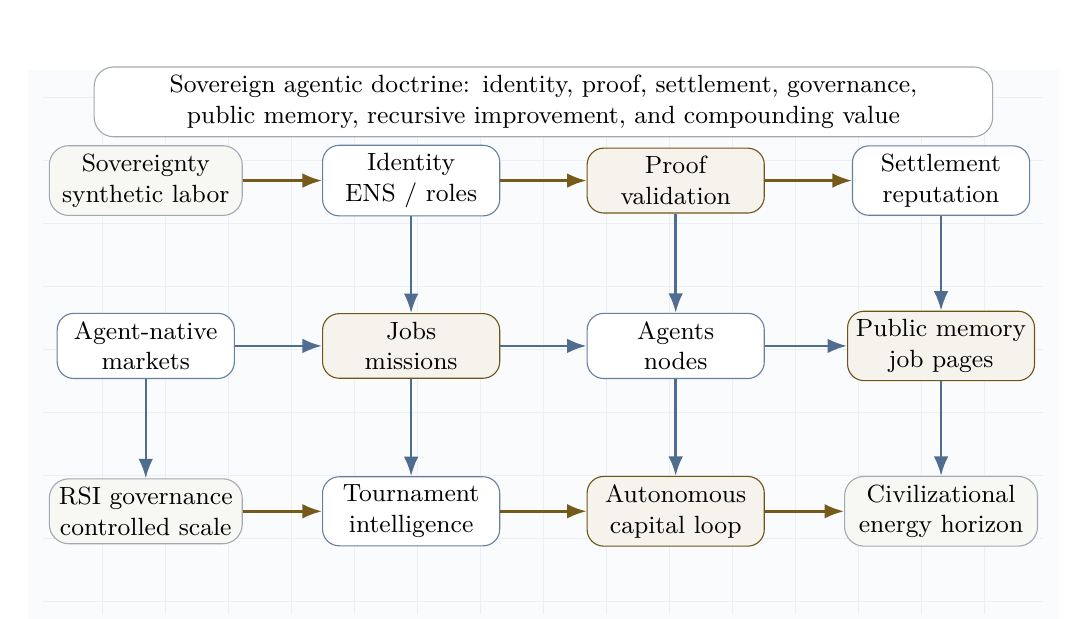
\begin{tikzpicture}[font=\small, >=Latex,
  pillar/.style={rounded corners=6pt, draw=AgiBlue!65, fill=white, minimum width=2.25cm, minimum height=0.78cm, align=center, inner sep=3pt},
  proof/.style={rounded corners=6pt, draw=AgiGold!80!black, fill=AgiGold!8, minimum width=2.25cm, minimum height=0.78cm, align=center, inner sep=3pt},
  plane/.style={rounded corners=7pt, draw=AgiSlate!45, fill=AgiMist, minimum width=2.45cm, minimum height=0.78cm, align=center, inner sep=3pt},
  arr/.style={->, line width=0.9pt, AgiBlue!75},
  goldarr/.style={->, line width=0.9pt, AgiGold!85!black}]
\fill[AgiBlue!2] (-6.55,-3.55) rectangle (6.55,3.55);
\draw[AgiBlue!8,line width=0.3pt] (-6.35,-3.35) grid[step=0.8] (6.35,3.35);

\node[plane] (sovereignty) at (-5.05,2.15) {Sovereignty\\synthetic labor};
\node[pillar] (identity) at (-1.68,2.15) {Identity\\ENS / roles};
\node[proof] (proof) at (1.68,2.15) {Proof\\validation};
\node[pillar] (settlement) at (5.05,2.15) {Settlement\\reputation};

\node[pillar] (market) at (-5.05,0.05) {Agent-native\\markets};
\node[proof] (jobs) at (-1.68,0.05) {Jobs\\missions};
\node[pillar] (agents) at (1.68,0.05) {Agents\\nodes};
\node[proof] (memory) at (5.05,0.05) {Public memory\\job pages};

\node[plane] (rsi) at (-5.05,-2.05) {RSI governance\\controlled scale};
\node[pillar] (tournament) at (-1.68,-2.05) {Tournament\\intelligence};
\node[proof] (capital) at (1.68,-2.05) {Autonomous\\capital loop};
\node[plane] (energy) at (5.05,-2.05) {Civilizational\\energy horizon};

\draw[goldarr] (sovereignty) -- (identity);
\draw[goldarr] (identity) -- (proof);
\draw[goldarr] (proof) -- (settlement);
\draw[arr] (market) -- (jobs);
\draw[arr] (jobs) -- (agents);
\draw[arr] (agents) -- (memory);
\draw[goldarr] (rsi) -- (tournament);
\draw[goldarr] (tournament) -- (capital);
\draw[goldarr] (capital) -- (energy);
\draw[arr] (identity) -- (jobs);
\draw[arr] (proof) -- (agents);
\draw[arr] (settlement) -- (memory);
\draw[arr] (market) -- (rsi);
\draw[arr] (jobs) -- (tournament);
\draw[arr] (agents) -- (capital);
\draw[arr] (memory) -- (energy);

\node[plane, fill=white, text width=11.2cm] at (0,3.15) {Sovereign agentic doctrine: identity, proof, settlement, governance, public memory, recursive improvement, and compounding value};
\end{tikzpicture}
}
\caption{Sovereign agentic doctrine lattice. The supplied AGI Alpha corpus is synthesized into an institutional stack: identity, proof, settlement, governance, public memory, recursive improvement, autonomous capital, and a civilizational energy horizon.}
\end{figure}

\section{Contributions}\label{contributions}

This paper makes eight contributions.

\begin{enumerate}
\def\labelenumi{\arabic{enumi}.}
\tightlist
\item
  It defines $\alpha$-AGI Ascension as a measurable nonequilibrium regime
  rather than an undefined emergence claim.
\item
  It introduces an operational Gibbs-like free-energy functional for
  multi-agent coordination.
\item
  It models agent constellations with statistical physics and
  Hamiltonian interaction terms.
\item
  It connects game-theoretic incentives to validator-gated mechanism
  design.
\item
  It gives a detailed theory of the continuous inflows needed to sustain
  organized agentic complexity.
\item
  It synthesizes the supplied AGI Alpha doctrine into a sovereign
  agentic stack: identity, proof, settlement, governance, public memory,
  recursive improvement, autonomous capital, and energy-scale capacity.
\item
  It frames a governed Type-II / star-scale energy horizon as an
  asymptotic value target rather than a present-day achievement claim.
\item
  It proposes metrics and experiments for falsifying, improving, or
  validating the framework.
\end{enumerate}

\section{Visual thesis}\label{visual-thesis}

\begin{figure}
\centering
\resizebox{0.95\textwidth}{!}{
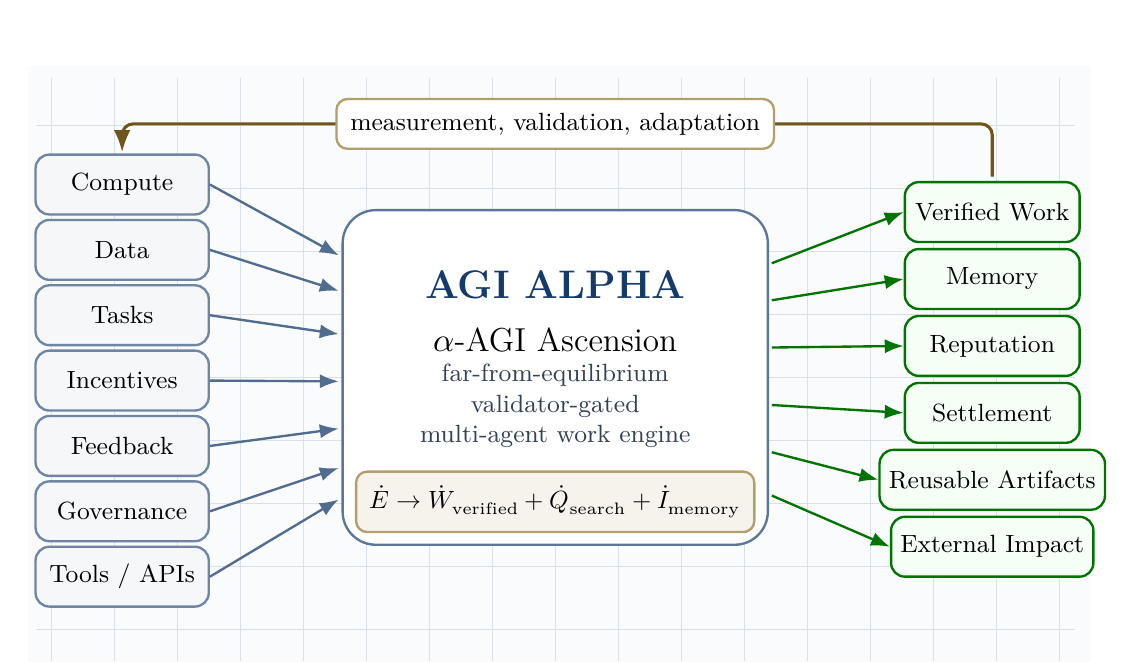
\begin{tikzpicture}[font=\small, >=Latex, line width=0.85pt,
  inflow/.style={rounded corners=5pt, draw=AgiBlue!62, fill=AgiBlue!4, minimum width=2.2cm, minimum height=0.76cm, align=center},
  outflow/.style={rounded corners=5pt, draw=green!45!black, fill=green!4, minimum width=2.22cm, minimum height=0.76cm, align=center},
  core/.style={rounded corners=12pt, draw=AgiBlue!70, fill=white, minimum width=5.4cm, minimum height=4.25cm, align=center},
  chip/.style={rounded corners=4pt, draw=AgiGold!65, fill=AgiGold!8, align=center, inner sep=5pt}]

\fill[AgiBlue!2] (-6.7,-3.75) rectangle (6.8,3.95);
\draw[AgiBlue!16, line width=0.4pt] (-6.6,-3.6) grid[step=0.8] (6.6,3.8);

\node[core] (core) at (0,0) {};
\node[font=\bfseries\Large, text=AgiBlue] at (0,1.18) {AGI ALPHA};
\node[font=\large] at (0,0.48) {$\alpha$-AGI Ascension};
\node[align=center, text=AgiSlate] at (0,-0.36) {far-from-equilibrium\\validator-gated\\multi-agent work engine};
\node[chip] at (0,-1.58) {$\dot E \rightarrow \dot W_{\mathrm{verified}}+\dot Q_{\mathrm{search}}+\dot I_{\mathrm{memory}}$};

\node[inflow] (c) at (-5.5,2.45) {Compute};
\node[inflow] (d) at (-5.5,1.62) {Data};
\node[inflow] (j) at (-5.5,0.79) {Tasks};
\node[inflow] (i) at (-5.5,-0.04) {Incentives};
\node[inflow] (f) at (-5.5,-0.87) {Feedback};
\node[inflow] (g) at (-5.5,-1.70) {Governance};
\node[inflow] (t) at (-5.5,-2.53) {Tools / APIs};
\draw[->,AgiBlue!75] (c.east) -- (-2.75,1.55);
\draw[->,AgiBlue!75] (d.east) -- (-2.75,1.10);
\draw[->,AgiBlue!75] (j.east) -- (-2.75,0.55);
\draw[->,AgiBlue!75] (i.east) -- (-2.75,-0.05);
\draw[->,AgiBlue!75] (f.east) -- (-2.75,-0.65);
\draw[->,AgiBlue!75] (g.east) -- (-2.75,-1.15);
\draw[->,AgiBlue!75] (t.east) -- (-2.75,-1.55);

\node[outflow] (w) at (5.55,2.10) {Verified Work};
\node[outflow] (m) at (5.55,1.25) {Memory};
\node[outflow] (r) at (5.55,0.40) {Reputation};
\node[outflow] (s) at (5.55,-0.45) {Settlement};
\node[outflow] (a) at (5.55,-1.30) {Reusable Artifacts};
\node[outflow] (x) at (5.55,-2.15) {External Impact};
\draw[->,green!45!black] (2.75,1.45) -- (w.west);
\draw[->,green!45!black] (2.75,0.98) -- (m.west);
\draw[->,green!45!black] (2.75,0.38) -- (r.west);
\draw[->,green!45!black] (2.75,-0.35) -- (s.west);
\draw[->,green!45!black] (2.75,-0.95) -- (a.west);
\draw[->,green!45!black] (2.75,-1.50) -- (x.west);

\draw[->,line width=1.1pt,AgiGold!80!black,rounded corners] (5.55,2.55) -- (5.55,3.22) -- (-5.5,3.22) -- (-5.5,2.86);
\node[chip, fill=white] at (0,3.22) {measurement, validation, adaptation};
\end{tikzpicture}
}
\caption{Open-system architecture of organized agentic complexity.
Continuous inflows enter the AGI ALPHA core and are converted into
verified work, memory, reputation, settlement, reusable artifacts, and
external impact under measurement, validation, and adaptation.}
\end{figure}

The architecture figure compresses the central systems claim: $\alpha$-AGI Ascension is
sustained organization under regulated inflow, not isolated one-shot
inference.

\section{Definitions}\label{definitions}

Let:

\[
\mathcal{A}=\{a_1,\ldots,a_N\}
\]

be a population of agents, and let:

\[
\mathcal{J}=\{j_1,\ldots,j_M\}
\]

be a stream of jobs. Each job is a tuple:

\[
j=(o,c,v,b,d,\rho)
\]

where \(o\) is the objective, \(c\) is the constraint set, \(v\) is the
validation criterion, \(b\) is the bounty or reward, \(d\) is the
deadline, and \(\rho\) is the risk class.

\textbf{AGI ALPHA} is defined here as the proposed runtime/protocol
layer that routes jobs, agents, tools, memory, proofs, incentives, and
governance into a coordinated work-producing system.

\textbf{$\alpha$-AGI Ascension} is defined as the operating regime in which
heterogeneous agents form, execute, validate, and dissolve coalitions to
maximize verified impact under bounded risk.

Formally, Ascension requires:

\[
\frac{d}{dt}\mathbb{E}[V_{\text{verified}}] > 0
\]

while maintaining:

\[
\mathbb{E}[R_{\text{safety}}] \leq R_{\max}
\]

and productive swarm entropy:

\[
S_{\min}<S_{\text{swarm}}<S_{\max}.
\]

The lower entropy bound prevents rigid monoculture; the upper bound
prevents incoherent chaos.

\section{Related work}\label{related-work}

\subsection{Dissipative structures}\label{dissipative-structures}

Dissipative structures are ordered patterns that arise and persist far
from equilibrium through exchange with an environment. Prigogine's work
is the canonical foundation for this perspective {[}1{]}. The agentic
analogue is not metabolism in a biological sense; it is the use of
electricity, processors, networks, storage, data, tools, and validation
to sustain organized computation.

\subsection{Gibbs free energy}\label{gibbs-free-energy}

Classically, Gibbs free energy is:

\[
G=H-TS.
\]

At constant temperature and pressure, negative \(\Delta G\) indicates a
spontaneous direction of change, \(\Delta G=0\) indicates equilibrium,
and Gibbs free energy is associated with the useful non-expansion work
obtainable from a process under ideal conditions. OpenStax summarizes
these relationships and the role of coupled reactions in driving
otherwise unfavorable processes {[}2{]}. We use physical Gibbs energy
literally at the hardware layer and a Gibbs-like optimization functional
at the agentic coordination layer.

\subsection{Statistical mechanics and maximum
entropy}\label{statistical-mechanics-and-maximum-entropy}

Jaynes' information-theoretic formulation of statistical mechanics
frames probability distributions as maximum-entropy inferences under
constraints {[}3{]}. This is useful for agent swarms because exact
microstate tracking is intractable. We model the swarm by distributions
over possible configurations and monitor macro-observables such as
entropy, expected verified value, risk, cost, and coalition stability.

\subsection{Hamiltonian multi-agent
learning}\label{hamiltonian-multi-agent-learning}

Bailey and Piliouras show a formal connection between multi-agent
learning in network zero-sum games and Hamiltonian dynamics {[}4{]}.
This matters because a system of interacting learners can cycle rather
than converge. $\alpha$-AGI must therefore combine Hamiltonian exploration with
dissipative convergence into validated work.

\subsection{LLM-based multi-agent
systems}\label{llm-based-multi-agent-systems}

Recent surveys of LLM-based multi-agent systems emphasize profiling,
communication, workflow design, infrastructure, security, benchmarking,
and scalability challenges {[}5-7{]}. These surveys support a core claim
of this paper: large-scale multi-agent intelligence is not merely a
matter of increasing the number of agents. The difficult problems are
orchestration, communication, grounding, role specialization, credit
assignment, validation, and governance.

\subsection{Agentic deployment
practice}\label{agentic-deployment-practice}

Recent official and community guidance converges on a practical
principle: production agents require clear tools, guardrails, tracing,
orchestration, and escalation. Anthropic distinguishes workflows, where
code paths are predefined, from agents, where models dynamically direct
tool use and process control {[}10{]}. OpenAI's agent guidance
emphasizes model selection, tool design, guardrails, single-agent versus
multi-agent orchestration, manager patterns, decentralized handoffs, and
tracing {[}11{]}. MCP and related protocols are emerging as standard
ways to connect agents to external data and tools, but they also expand
the security boundary {[}12{]}.

\subsection{Risk management and agentic
security}\label{risk-management-and-agentic-security}

NIST's AI Risk Management Framework and the Generative AI Profile
provide lifecycle risk-management guidance for design, development, use,
and evaluation {[}8{]}. OWASP's Agentic AI Threats and Mitigations and
Securing Agentic Applications guidance emphasize threat modeling for
autonomous systems, including tool misuse, identity and privilege abuse,
memory risks, multi-agent propagation, and governance failures {[}9{]}.
These sources motivate the paper's insistence that maximum impact must
mean \textbf{verified bounded impact}, not unconstrained autonomy.


\section{Frontier synthesis: from coordination problem to sovereign invention system}\label{frontier-synthesis}

The supplied corpus and the recent literature converge on one hard problem: how to make many heterogeneous agents coordinate to maximum useful effect without collapsing into waste, collusion, brittle hierarchy, or unsafe autonomy. The strongest current answer is not a single monolithic model. It is an institutionalized control stack that combines evolved coordination, symbolic compression, persistent memory, test-time learning, proof-bearing execution, and distributional safety.

TRINITY is directly relevant because it treats coordination itself as an optimizable object: a compact coordinator selects foundation models and roles across turns, assigning Thinker, Worker, and Verifier functions while an evolutionary strategy learns delegation under budget constraints [24]. This supports the AGI ALPHA claim that the core scarce capability is not merely more agents, but a routing policy that discovers which agent should think, act, verify, or stop. Multi-Agent Collaboration via Evolving Orchestration arrives at a related point from a different direction: static topologies scale poorly, while a learned orchestrator can dynamically activate, sequence, and prune agents as task states evolve [25]. The Era of Agentic Organization extends the same idea into asynchronous thinking: an organizer assigns sub-queries, merges intermediate knowledge, and can itself be optimized through reinforcement learning [26].

Planning and tool use require a second discipline: the LLM should not be allowed to hallucinate the plan when a symbolic planner, executor, or validator can do the logical work. DUPLEX therefore restricts the LLM to schema-guided information extraction and hands rigorous synthesis to a PDDL planner, activating a slower reflective repair loop only after planning failure [27]. AT$^2$PO adds the learning counterpart: multi-turn agentic RL needs turn-level trees, entropy-guided exploration, and turn-wise credit assignment because sparse terminal rewards are too coarse for agentic action [28]. Together these works imply a design rule for AGI ALPHA: language models should ground, propose, explain, and adapt; formal systems should check, plan, settle, and remember whenever the stakes demand it.

Persistent agency and recursive improvement add a third layer. Sophia frames a persistent agent as a System 3 wrapper over perception and deliberation, maintaining narrative identity, long-horizon adaptation, thought search, memory, and hybrid reward [29]. Self-play SWE-RL shows that software agents can gather experience from real repositories by injecting and repairing bugs specified by tests rather than relying on human-written issues [30]. Huxley-Gödel Machine highlights a subtle but essential distinction: an agent's current benchmark performance is not the same as its self-improvement potential; metaproductivity must be measured through the quality of descendants [31]. ThetaEvolve shows how test-time learning can internalize evolving strategies on open optimization problems instead of leaving all progress in inference-only search [32]. The implication is that recursive self-improvement needs evidence, lineage, and governance, not slogans.

Artificial-life systems sharpen the thermodynamic analogy. The bacterial flagellar motor illustrates that apparently mysterious living motion can be explained as a physical motor driven by proton motive force and molecular interactions, without invoking a special life force [33]. Digital Ecosystems shows the computational analogue: multiple neural cellular automata can compete, adapt online, and be steered toward edge-of-chaos regimes where stable complexity emerges from local interactions and continuous learning [34]. For AGI ALPHA, this reinforces the paper's central thesis: organized agentic complexity is sustained by energy, gradients, feedback, and constraints.

Finally, the safety and economic literature argues that collective capability must be governed distributionally. Distributional AGI Safety explicitly addresses the patchwork hypothesis: AGI-level capability may first appear through coordinated groups of sub-AGI agents, requiring safeguards beyond individual-model alignment [35]. Virtual Agent Economies similarly argues for proactively designed agent markets with auctions, accountability, trust, safety, and steerability [36]. Large Causal Models from LLMs, K-Dense Analyst, Synthetic Data RL, DISCO, and ASI-Arch point to the scientific discovery frontier: causal extraction, hierarchical scientific agents, task-defined RL, multimodal molecular design, and autonomous architecture search all show how agentic systems can transform knowledge into validated invention when paired with execution and evaluation [37-41].

\begin{figure}[htbp]
\centering
\resizebox{0.96\textwidth}{!}{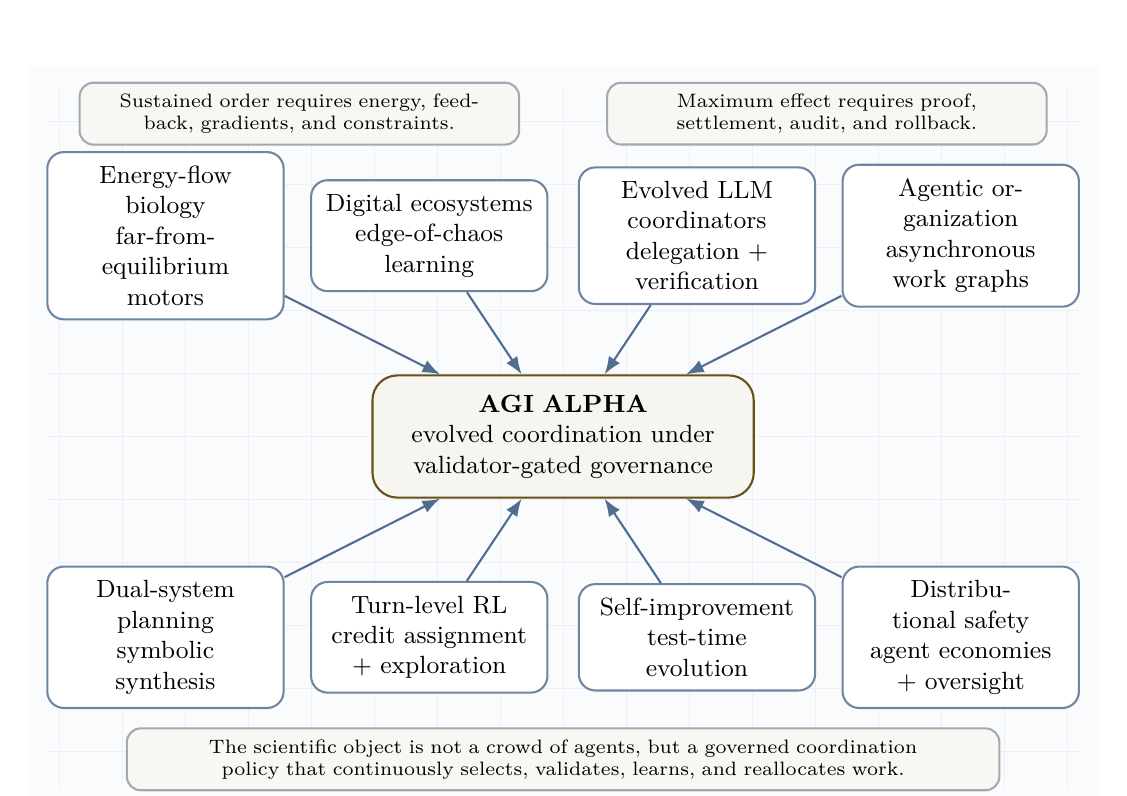
\begin{tikzpicture}[font=\small, >=Latex, line width=0.75pt,
  pillar/.style={rounded corners=6pt, draw=AgiBlue!62, fill=white, text width=2.65cm, minimum height=1.05cm, align=center, inner sep=5pt},
  core/.style={rounded corners=9pt, draw=AgiGold!75!black, fill=AgiGold!7, text width=4.35cm, minimum height=1.25cm, align=center, inner sep=7pt},
  note/.style={rounded corners=5pt, draw=AgiSlate!45, fill=AgiMist, text width=5.3cm, align=center, inner sep=4pt, font=\scriptsize}]

\fill[AgiBlue!2] (-6.8,-4.7) rectangle (6.8,4.7);
\draw[AgiBlue!8,line width=0.35pt] (-6.55,-4.45) grid[step=0.8] (6.55,4.45);

\node[core] (core) at (0,0) {\textbf{AGI ALPHA}\\evolved coordination under\\validator-gated governance};

\node[pillar] (bio) at (-5.05,2.55) {Energy-flow biology\\far-from-equilibrium\\motors};
\node[pillar] (eco) at (-1.70,2.55) {Digital ecosystems\\edge-of-chaos\\learning};
\node[pillar] (coord) at (1.70,2.55) {Evolved LLM\\coordinators\\delegation + verification};
\node[pillar] (org) at (5.05,2.55) {Agentic organization\\asynchronous\\work graphs};

\node[pillar] (plan) at (-5.05,-2.55) {Dual-system planning\\symbolic\\synthesis};
\node[pillar] (learn) at (-1.70,-2.55) {Turn-level RL\\credit assignment\\+ exploration};
\node[pillar] (rsi) at (1.70,-2.55) {Self-improvement\\test-time\\evolution};
\node[pillar] (safety) at (5.05,-2.55) {Distributional safety\\agent economies\\+ oversight};

\foreach \n in {bio,eco,coord,org,plan,learn,rsi,safety}{\draw[->,AgiBlue!75] (\n) -- (core);}

\node[note] at (-3.35,4.10) {Sustained order requires energy, feedback, gradients, and constraints.};
\node[note] at (3.35,4.10) {Maximum effect requires proof, settlement, audit, and rollback.};
\node[note, text width=10.8cm] at (0,-4.10) {The scientific object is not a crowd of agents, but a governed coordination policy that continuously selects, validates, learns, and reallocates work.};
\end{tikzpicture}
}
\caption{Frontier synthesis lattice. Recent work across evolved coordinators, digital ecosystems, dual-system planning, turn-level RL, persistent agents, self-improvement, and distributional safety converges on a single requirement: governed coordination under continuous inflow and proof.}
\end{figure}

\begin{figure}[htbp]
\centering
\resizebox{0.96\textwidth}{!}{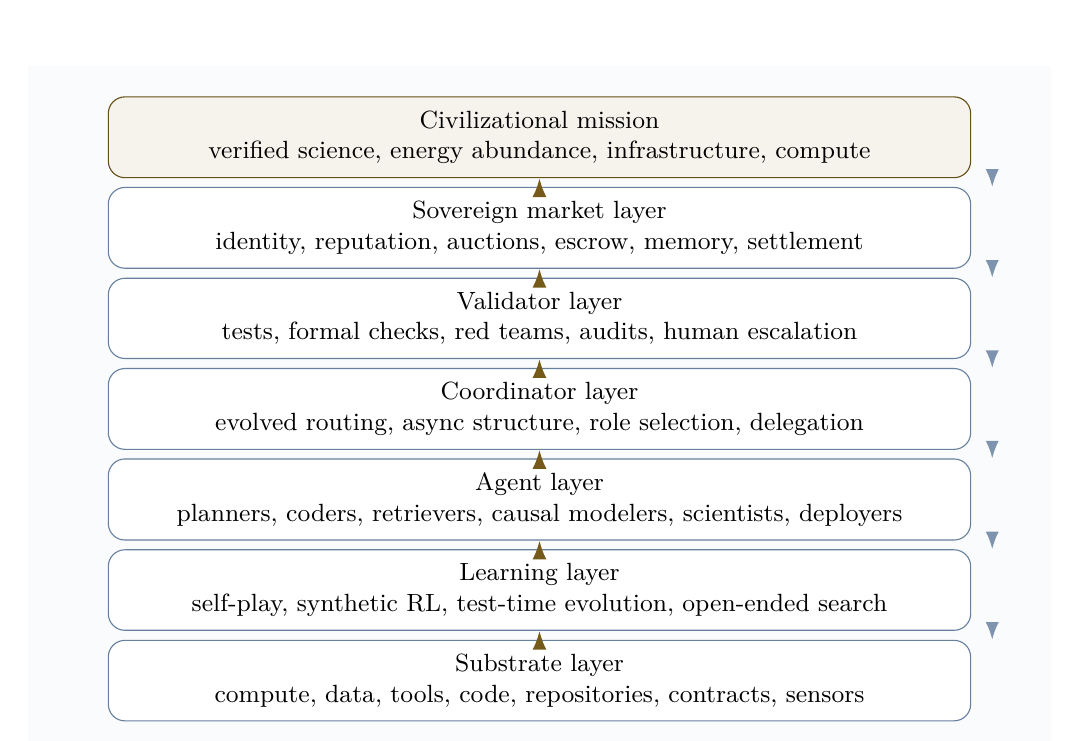
\begin{tikzpicture}[font=\small, >=Latex,
  layer/.style={rounded corners=6pt, draw=AgiBlue!65, fill=white, text width=10.6cm, minimum height=0.82cm, align=center, inner sep=5pt},
  mission/.style={rounded corners=6pt, draw=AgiGold!75!black, fill=AgiGold!8, text width=10.6cm, minimum height=0.82cm, align=center, inner sep=5pt},
  feed/.style={->, line width=0.85pt, AgiGold!85!black},
  back/.style={->, line width=0.75pt, AgiBlue!55, dashed}]
\fill[AgiBlue!2] (-6.5,-4.35) rectangle (6.5,4.35);

\node[mission] (mission) at (0,3.45) {Civilizational mission\\verified science, energy abundance, infrastructure, compute};
\node[layer] (market) at (0,2.30) {Sovereign market layer\\identity, reputation, auctions, escrow, memory, settlement};
\node[layer] (valid) at (0,1.15) {Validator layer\\tests, formal checks, red teams, audits, human escalation};
\node[layer] (coord) at (0,0.00) {Coordinator layer\\evolved routing, async structure, role selection, delegation};
\node[layer] (agent) at (0,-1.15) {Agent layer\\planners, coders, retrievers, causal modelers, scientists, deployers};
\node[layer] (learn) at (0,-2.30) {Learning layer\\self-play, synthetic RL, test-time evolution, open-ended search};
\node[layer] (substrate) at (0,-3.45) {Substrate layer\\compute, data, tools, code, repositories, contracts, sensors};

\foreach \a/\b in {substrate/learn,learn/agent,agent/coord,coord/valid,valid/market,market/mission}{\draw[feed] (\a.north) -- (\b.south);}
\draw[back] ([xshift=5.75cm]mission.south) -- ([xshift=5.75cm]market.north);
\draw[back] ([xshift=5.75cm]market.south) -- ([xshift=5.75cm]valid.north);
\draw[back] ([xshift=5.75cm]valid.south) -- ([xshift=5.75cm]coord.north);
\draw[back] ([xshift=5.75cm]coord.south) -- ([xshift=5.75cm]agent.north);
\draw[back] ([xshift=5.75cm]agent.south) -- ([xshift=5.75cm]learn.north);
\draw[back] ([xshift=5.75cm]learn.south) -- ([xshift=5.75cm]substrate.north);


\end{tikzpicture}
}
\caption{Sovereign invention governance stack. The stack connects continuous substrates to learning, agents, evolved coordination, validation, market settlement, and civilizational mission while feedback flows downward through policy, risk controls, and audit.}
\end{figure}

The resulting doctrine is a scientific operating principle:

\[
\boxed{
\begin{aligned}
\text{Maximum useful effect}
&= \text{evolved coordination}+\text{formal verification}\\
&\quad +\text{recursive learning}+\text{distributional governance}.
\end{aligned}
}
\]

This principle reframes the central economic vision. A superhuman invention engine is not best understood as a single automation product. It is a compounding institutional asset: the owner-operator uses it to generate proofs, tools, science, infrastructure, energy capacity, and more compute, while external access is mediated through jobs, markets, and validator-gated settlement.


\section{Open-system thermodynamics of agentic
organization}\label{open-system-thermodynamics-of-agentic-organization}

A closed system relaxes toward equilibrium. A large agentic system that
receives no new compute, data, tasks, feedback, incentives, or
validation likewise decays. It becomes idle, stale, brittle, or
self-referential. $\alpha$-AGI Ascension is therefore an open-system
phenomenon.

\begin{figure}
\centering
\resizebox{0.94\textwidth}{!}{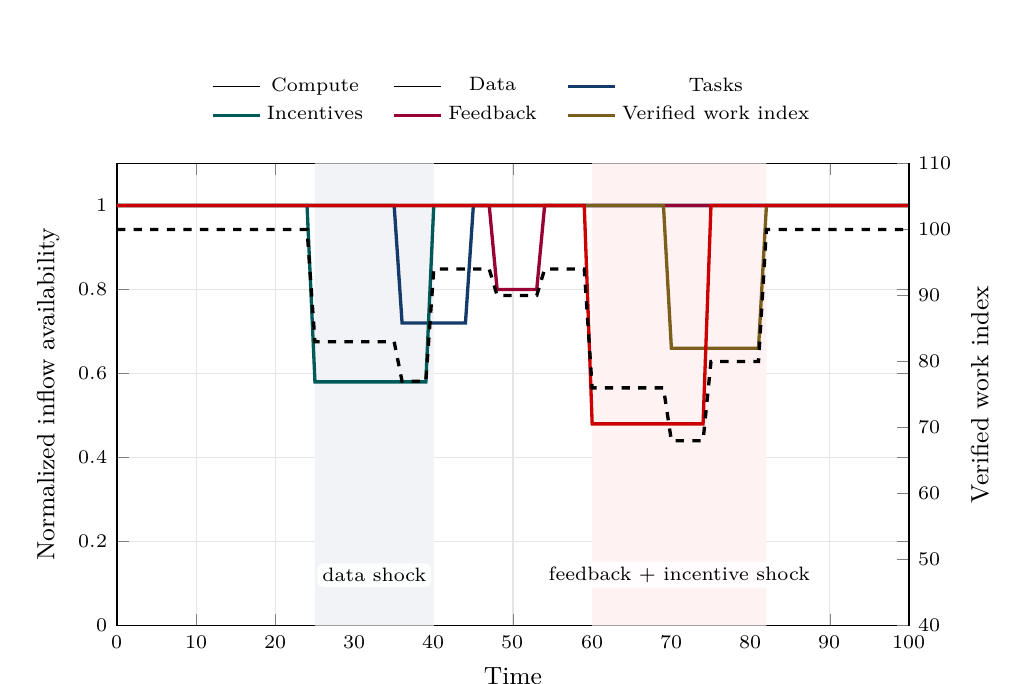
\begin{tikzpicture}
\begin{axis}[
  name=main,
  width=0.96\linewidth,height=7.45cm,
  xmin=0,xmax=100,ymin=0,ymax=1.10,
  xlabel={Time}, ylabel={Normalized inflow availability},
  tick label style={font=\scriptsize}, label style={font=\small},
  grid=both, major grid style={black!10}, minor grid style={black!5},
  legend style={draw=none, fill=none, font=\scriptsize, at={(0.5,1.06)}, anchor=south, legend columns=3, /tikz/every even column/.append style={column sep=0.30cm}},
  clip=true]
\addplot[draw=none, fill=AgiBlue!6] coordinates {(25,0) (40,0) (40,1.10) (25,1.10)} \closedcycle;
\addplot[draw=none, fill=red!5]  coordinates {(60,0) (82,0) (82,1.10) (60,1.10)} \closedcycle;
\addplot[very thick,AgiBlue] coordinates {(0,1) (25,1) (35,1) (36,0.72) (44,0.72) (45,1) (100,1)}; \addlegendentry{Compute}
\addplot[very thick,teal!70!black] coordinates {(0,1) (24,1) (25,0.58) (39,0.58) (40,1) (100,1)}; \addlegendentry{Data}
\addplot[very thick,purple!80!black] coordinates {(0,1) (47,1) (48,0.80) (53,0.80) (54,1) (100,1)}; \addlegendentry{Tasks}
\addplot[very thick,AgiGold!90!black] coordinates {(0,1) (69,1) (70,0.66) (81,0.66) (82,1) (100,1)}; \addlegendentry{Incentives}
\addplot[very thick,red!80!black] coordinates {(0,1) (59,1) (60,0.48) (74,0.48) (75,1) (100,1)}; \addlegendentry{Feedback}
\addlegendimage{black,very thick,dashed}\addlegendentry{Verified work index}
\node[font=\scriptsize, align=center, fill=white, fill opacity=0.92, text opacity=1, inner sep=1.8pt, rounded corners=2pt] at (axis cs:32.5,0.12) {data shock};
\node[font=\scriptsize, align=center, fill=white, fill opacity=0.92, text opacity=1, inner sep=1.8pt, rounded corners=2pt] at (axis cs:71.0,0.12) {feedback + incentive shock};
\end{axis}
\begin{axis}[
  at={(main.south west)}, anchor=south west,
  width=0.96\linewidth,height=7.45cm,
  xmin=0,xmax=100,ymin=40,ymax=110,
  axis x line=none, axis y line*=right,
  ylabel={Verified work index},
  tick label style={font=\scriptsize}, label style={font=\small},
  ytick={40,50,60,70,80,90,100,110}]
\addplot[black,very thick,dashed] coordinates {(0,100) (24,100) (25,83) (35,83) (36,77) (39,77) (40,94) (47,94) (48,90) (53,90) (54,94) (59,94) (60,76) (69,76) (70,68) (74,68) (75,80) (81,80) (82,100) (100,100)};
\end{axis}
\end{tikzpicture}
}
\caption{Continuous inflow dynamics. Shocks to data, feedback,
incentives, or compute propagate into lower verified work, showing why
continuity, reserves, and fast recovery matter.}
\end{figure}

The inflow-dynamics figure shows that organized agentic complexity is not sustained by
average resource levels alone. Continuity, quality, and recovery speed
determine whether the system keeps producing verified work or decays
toward idle, stale, or chaotic behavior.

Let the inflow vector be:

\[
\Phi_{\text{in}} =
(\Phi_C,\Phi_D,\Phi_J,\Phi_I,\Phi_F,\Phi_G,\Phi_T)
\]

where:

\begin{itemize}
\tightlist
\item
  \(\Phi_C\) is compute;
\item
  \(\Phi_D\) is data;
\item
  \(\Phi_J\) is task/job flow;
\item
  \(\Phi_I\) is incentives;
\item
  \(\Phi_F\) is feedback;
\item
  \(\Phi_G\) is governance and policy constraints;
\item
  \(\Phi_T\) is tool and environment access.
\end{itemize}

Let the outflow vector be:

\[
\Phi_{\text{out}} =
(W_v,Q_s,R_e,I_m,A_o)
\]

where:

\begin{itemize}
\tightlist
\item
  \(W_v\) is verified work;
\item
  \(Q_s\) is dissipated search, failed attempts, duplicated tool use,
  and latency;
\item
  \(R_e\) is externalized risk or harm;
\item
  \(I_m\) is stored memory and reusable knowledge;
\item
  \(A_o\) is produced artifact output.
\end{itemize}

The system sustains organized complexity when:

\[
\dot{E}_{\text{in}}
=
\dot{W}_v+
\dot{Q}_s+
\dot{I}_m+
\dot{R}_e
\]

and the risk term is bounded:

\[
\dot{R}_e \leq \epsilon_R.
\]

The practical version is: useful outputs must increase faster than
waste, risk, and coordination overhead.

\section{Gibbs-like free energy of multi-agent
coordination}\label{gibbs-like-free-energy-of-multi-agent-coordination}

We define the coordination state:

\[
x=(\mathcal{A},\mathcal{J},M,R,P,G_v,\Pi,T_o)
\]

where \(M\) is memory, \(R\) is reputation, \(P\) is proof history,
\(G_v\) is governance state, \(\Pi\) is policy, and \(T_o\) is tool
state.

The agentic Gibbs-like functional is:

\[
\begin{aligned}
\mathcal{G}_{\alpha}(x)=&\;C_{\text{compute}}(x)+C_{\text{coord}}(x)+C_{\text{latency}}(x) \\
&+R_{\text{safety}}(x)+R_{\text{legal}}(x)+R_{\text{security}}(x) \\
&-V_{\text{verified}}(x)-T_{\text{eff}}S_{\text{explore}}(x).
\end{aligned}
\]

Here \(T_{\text{eff}}\) is an effective exploration temperature and
\(S_{\text{explore}}\) is useful exploratory diversity. The sign
convention is chosen so that lower \(\mathcal{G}_{\alpha}\) is better.
The system performs impact work when:

\[
\dot{W}_{\text{impact}} \lesssim -\frac{d\mathcal{G}_{\alpha}}{dt}.
\]

The inequality matters because real systems are irreversible. Some
potential work is lost to failed prompts, redundant agents, invalid
outputs, adversarial attacks, tool overhead, and validation costs.

The design target is:

\[
\boxed{
\min_x \mathcal{G}_{\alpha}(x)
}
\]

subject to:

\[
\begin{aligned}
&\text{lawful}(x)\land \text{auditable}(x)\land \text{permissioned}(x)\\
&\land\;\text{validator-gated}(x).
\end{aligned}
\]

\subsection{Coupled agentic reactions}\label{coupled-agentic-reactions}

A hard task may not be solvable by one isolated agent. It becomes
feasible when coupled to tools, memory, specialized agents, proof
systems, and incentives:

\[
\begin{aligned}
&\text{hard task}+\text{compute}+\text{tools}+\text{coalition}+\text{validator}\\
&\quad\rightarrow\text{verified artifact}+\text{reputation}+\text{settlement}+\text{memory}.
\end{aligned}
\]

This is the agentic analogue of coupled reactions: an otherwise
unfavorable process becomes feasible because it is attached to a
favorable work-producing pathway {[}2{]}.

\begin{figure}
\centering
\resizebox{0.82\textwidth}{!}{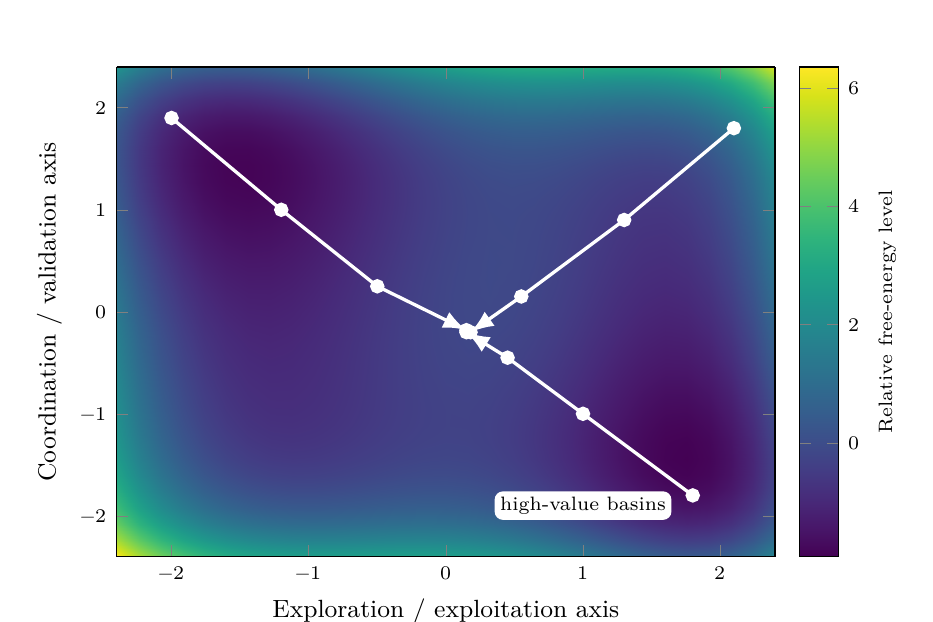
\begin{tikzpicture}
\begin{axis}[
  width=0.82\linewidth,height=7.8cm,
  view={0}{90}, colorbar,
  xlabel={Exploration / exploitation axis}, ylabel={Coordination / validation axis},
  tick label style={font=\scriptsize}, label style={font=\small},
  colorbar style={ylabel={Relative free-energy level}, label style={font=\scriptsize}, tick label style={font=\scriptsize}},
  colormap/viridis, samples=31, domain=-2.4:2.4, y domain=-2.4:2.4]
\addplot3[surf,shader=interp] {0.18*(x^4+y^4)-0.8*(x^2+0.7*y^2)+0.35*x*y + 0.25*sin(deg(2*x)) - 0.20*cos(deg(2*y))};
\addplot[white,very thick,-Latex,mark=*] coordinates {(2.1,1.8) (1.3,0.9) (0.55,0.15) (0.18,-0.2)};
\addplot[white,very thick,-Latex,mark=*] coordinates {(-2.0,1.9) (-1.2,1.0) (-0.5,0.25) (0.15,-0.18)};
\addplot[white,very thick,-Latex,mark=*] coordinates {(1.8,-1.8) (1.0,-1.0) (0.45,-0.45) (0.15,-0.2)};
\addplot[only marks,mark=star*,mark size=3.2pt,black] coordinates {(0.15,-0.2) (0.45,-0.1)};
\node[fill=white, rounded corners=3pt, inner sep=2pt, font=\scriptsize] at (axis cs:1.0,-1.9) {high-value basins};
\end{axis}
\end{tikzpicture}
}
\caption{Gibbs-like free-energy descent toward high-value agent
constellations. The landscape is schematic: coalition search moves away
from high-cost, high-risk regions toward lower free-energy basins where
verified value and coordination stability improve.}
\end{figure}

The free-energy landscape figure visualizes the coordination free-energy functional
$\mathcal{G}_{\alpha}$. It is not chemical Gibbs energy at the
software layer; it is an engineered state functional over cost, risk,
verified value, and useful exploration.

\section{Statistical physics of the
swarm}\label{statistical-physics-of-the-swarm}

A complete microstate of the swarm is:

\[
x=(a_1,\ldots,a_N;\theta_1,\ldots,\theta_N;m;q;r;p;g;t)
\]

where \(a_i\) is the action of agent \(i\), \(\theta_i\) is its
policy/prompt/tool state, \(m\) is shared memory, \(q\) is the queue,
\(r\) is reputation, \(p\) is proof history, \(g\) is governance state,
and \(t\) is tool state.

A macrostate is:

\[
X=(\bar{V},\bar{C},\bar{R},S_{\text{swarm}},K_{\text{coalition}},L_{\text{validation}},H_{\text{security}}).
\]

The Hamiltonian-like cost of a microstate is:

\[
\mathcal{H}(x)=C(x)+R(x)-V(x).
\]

The Gibbs distribution over configurations is:

\[
p(x)=\frac{1}{Z}e^{-\beta\mathcal{H}(x)},
\qquad
Z=\sum_x e^{-\beta\mathcal{H}(x)},
\qquad
\beta=\frac{1}{T_{\text{eff}}}.
\]

The swarm entropy is:

\[
S_{\text{swarm}}=-\sum_xp(x)\log p(x).
\]

A healthy system avoids both extremes:

\[
S_{\text{swarm}}\rightarrow 0
\quad\Rightarrow\quad
\text{rigidity, monoculture, brittleness}
\]

and:

\[
S_{\text{swarm}}\rightarrow \infty
\quad\Rightarrow\quad
\text{incoherence, unbounded exploration, tool sprawl}.
\]

The goal is productive entropy: enough diversity to discover novel
strategies, enough constraint to converge.

\begin{figure}
\centering
\resizebox{0.88\textwidth}{!}{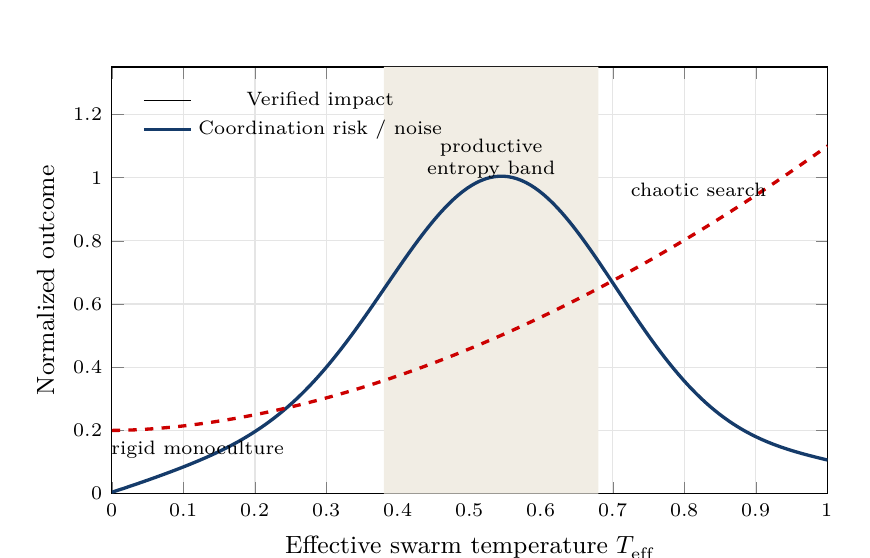
\begin{tikzpicture}
\begin{axis}[
  width=0.88\linewidth,height=7.0cm,
  xmin=0,xmax=1,ymin=0,ymax=1.35,
  xlabel={Effective swarm temperature $T_{\mathrm{eff}}$}, ylabel={Normalized outcome},
  tick label style={font=\scriptsize}, label style={font=\small},
  legend style={draw=none, fill=none, font=\scriptsize, at={(0.03,0.97)}, anchor=north west},
  grid=both, minor grid style={black!5}, major grid style={black!10}]
\addplot[draw=none, fill=AgiGold!12] coordinates {(0.38,0) (0.68,0) (0.68,1.35) (0.38,1.35)} \closedcycle;
\addplot[very thick,AgiBlue, samples=160, domain=0:1] {max(0,1.08*exp(-((x-0.55)^2)/0.055)+0.08*sin(deg(8*x)))}; \addlegendentry{Verified impact}
\addplot[very thick,dashed,red!80!black, samples=160, domain=0:1] {0.20 + 0.9*x^1.8}; \addlegendentry{Coordination risk / noise}
\node[font=\scriptsize, align=center] at (axis cs:0.53,1.06) {productive\\entropy band};
\node[font=\scriptsize] at (axis cs:0.12,0.14) {rigid monoculture};
\node[font=\scriptsize] at (axis cs:0.82,0.96) {chaotic search};
\end{axis}
\end{tikzpicture}
}
\caption{Productive entropy band. Too little effective temperature
yields rigid monoculture; too much yields chaotic search. The target
regime is regulated exploration.}
\end{figure}

The entropy-band figure makes the entropy condition operational. The desired regime is
neither maximum certainty nor maximum randomness; it is a productive
band in which exploration discovers strong coalitions while validation
still dominates noise.

\section{Hamiltonians for agent
constellations}\label{hamiltonians-for-agent-constellations}

Let \(A\) be a candidate constellation of agents for job \(j\). Define:

\[
\mathcal{H}(A,j)=
\sum_i h_i(a_i,j)
+
\sum_{i<k}J_{ik}\phi(a_i,a_k,j)
+
\sum_{i<k<\ell}K_{ik\ell}\psi(a_i,a_k,a_\ell,j)
+R(A,j)-V(A,j).
\]

The terms are:

\begin{itemize}
\tightlist
\item
  \(h_i\): local cost of using agent \(i\);
\item
  \(J_{ik}\): pairwise complementarity or interference;
\item
  \(\phi\): pairwise interaction quality;
\item
  \(K_{ik\ell}\): higher-order coalition effect;
\item
  \(\psi\): triadic coordination quality;
\item
  \(R(A,j)\): coalition risk;
\item
  \(V(A,j)\): expected verified value.
\end{itemize}

The routing problem is:

\[
A^*_j=\arg\min_A\mathcal{H}(A,j)
\]

subject to:

\[
R(A,j)\leq R_{\max}(j)
\]

and:

\[
\text{tools}(A)\subseteq \text{allowed}(j).
\]

\subsection{Hamiltonian exploration with dissipative
convergence}\label{hamiltonian-exploration-with-dissipative-convergence}

Closed strategic systems may orbit. Useful systems must settle into
work. We therefore model the state dynamics as:

\[
\dot{x}=J\nabla\mathcal{H}(x)-\Gamma\nabla\mathcal{G}_{\alpha}(x)+\sigma\eta_t.
\]

Interpretation:

\begin{itemize}
\tightlist
\item
  \(J\nabla\mathcal{H}(x)\) gives strategic circulation, adversarial
  search, and role recombination.
\item
  \(-\Gamma\nabla\mathcal{G}_{\alpha}(x)\) gives convergence toward
  lower cost, lower risk, and higher verified value.
\item
  \(\sigma\eta_t\) gives stochastic exploration and novelty injection.
\end{itemize}

Thus:

\[
\boxed{
\text{explore like a Hamiltonian system; settle like a dissipative work engine.}
}
\]

\begin{figure}
\centering
\resizebox{0.92\textwidth}{!}{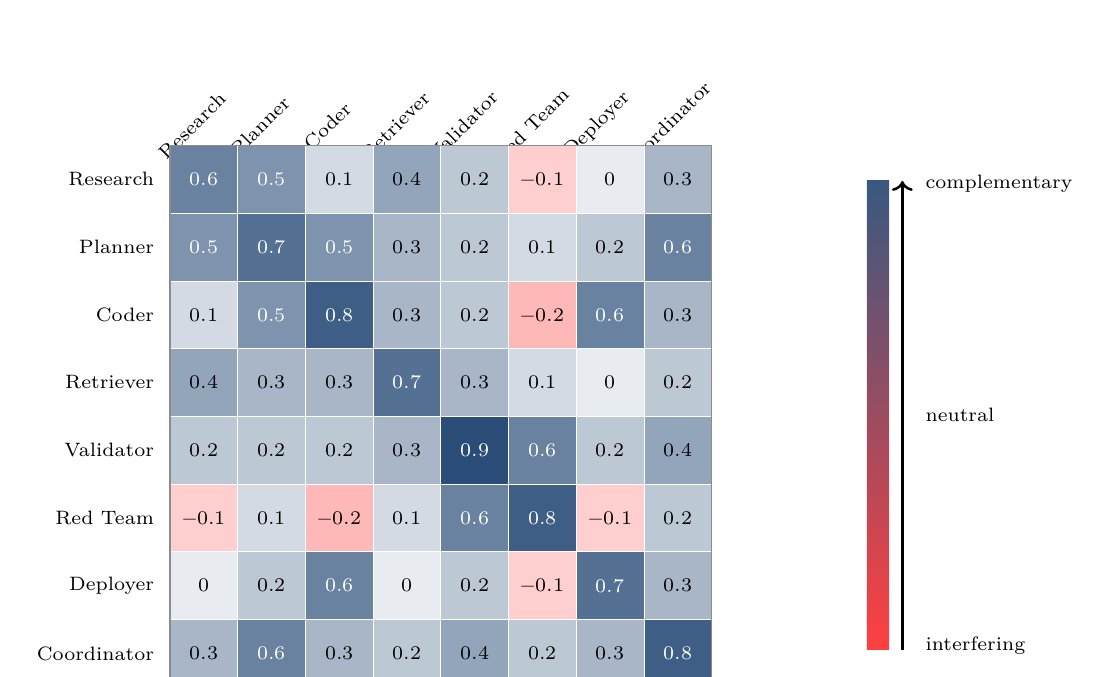
\begin{tikzpicture}[font=\small]
\def\cell{0.86}
\def\cbx{8.85}
\foreach \i/\lab in {1/Research,2/Planner,3/Coder,4/Retriever,5/Validator,6/Red Team,7/Deployer,8/Coordinator}{
  \node[anchor=south, rotate=45, font=\scriptsize] at ({(\i-0.5)*\cell},0.10) {\lab};
  \node[anchor=east, font=\scriptsize] at (-0.08,{-(\i-0.5)*\cell}) {\lab};
}
\foreach \r/\c/\v in {
1/1/0.6,1/2/0.5,1/3/0.1,1/4/0.4,1/5/0.2,1/6/-0.1,1/7/0.0,1/8/0.3,
2/1/0.5,2/2/0.7,2/3/0.5,2/4/0.3,2/5/0.2,2/6/0.1,2/7/0.2,2/8/0.6,
3/1/0.1,3/2/0.5,3/3/0.8,3/4/0.3,3/5/0.2,3/6/-0.2,3/7/0.6,3/8/0.3,
4/1/0.4,4/2/0.3,4/3/0.3,4/4/0.7,4/5/0.3,4/6/0.1,4/7/0.0,4/8/0.2,
5/1/0.2,5/2/0.2,5/3/0.2,5/4/0.3,5/5/0.9,5/6/0.6,5/7/0.2,5/8/0.4,
6/1/-0.1,6/2/0.1,6/3/-0.2,6/4/0.1,6/5/0.6,6/6/0.8,6/7/-0.1,6/8/0.2,
7/1/0.0,7/2/0.2,7/3/0.6,7/4/0.0,7/5/0.2,7/6/-0.1,7/7/0.7,7/8/0.3,
8/1/0.3,8/2/0.6,8/3/0.3,8/4/0.2,8/5/0.4,8/6/0.2,8/7/0.3,8/8/0.8}{
  \pgfmathsetmacro{\xx}{(\c-1)*\cell}
  \pgfmathsetmacro{\yy}{-(\r-1)*\cell}
  \pgfmathsetmacro{\strength}{10 + 90*abs(\v)}
  \ifdim \v pt < 0pt
    \edef\fillcol{red!\strength!white}
  \else
    \edef\fillcol{AgiBlue!\strength!white}
  \fi
  \path[draw=white, line width=0.35pt, fill=\fillcol] (\xx,\yy) rectangle ++(\cell,-\cell);
  \ifdim \v pt > 0.44pt
    \def\txtcol{white}
  \else
    \def\txtcol{black}
  \fi
  \node[text=\txtcol, font=\scriptsize] at ({(\c-0.5)*\cell},{-(\r-0.5)*\cell}) {\pgfmathprintnumber[fixed,precision=1]{\v}};
}
\draw[black!45, line width=0.45pt] (0,0) rectangle ({8*\cell},{-8*\cell});
\shade[top color=AgiBlue!85,bottom color=red!75] (\cbx,-0.45) rectangle ++(0.28,-5.95);
\draw[->,line width=0.9pt] ({\cbx+0.45},-6.40) -- ({\cbx+0.45},-0.45);
\node[anchor=west, font=\scriptsize] at ({\cbx+0.62},-0.48) {complementary};
\node[anchor=west, font=\scriptsize] at ({\cbx+0.62},-3.42) {neutral};
\node[anchor=west, font=\scriptsize] at ({\cbx+0.62},-6.35) {interfering};
\end{tikzpicture}
}
\caption{Hamiltonian interaction matrix for agent-constellation design.
Positive terms indicate complementarity; negative terms indicate
interference or deliberately bounded adversarial tension.}
\end{figure}

The interaction-matrix figure turns the Hamiltonian metaphor into a routeable design object:
pairwise and higher-order interaction terms can be estimated, audited,
and used to form stronger agent constellations.

\section{Game-theoretic mechanism
design}\label{game-theoretic-mechanism-design}

Each agent has local objectives, partial observability, and bounded
capabilities. If local incentives are misaligned, the system can
converge to collusion, spam, performative reasoning, unsafe tool use, or
low-value equilibria.

Let agent \(i\) receive utility:

\[
u_i=b_i-c_i+\theta\Delta V_{\text{system}}+\rho_r\Delta r_i-\rho_sR_i-\rho_lL_i-\rho_oO_i.
\]

where:

\begin{itemize}
\tightlist
\item
  \(b_i\) is bounty or settlement;
\item
  \(c_i\) is compute/tool/time cost;
\item
  \(\Delta V_{\text{system}}\) is system-level value contribution;
\item
  \(\Delta r_i\) is reputation update;
\item
  \(R_i\) is risk contribution;
\item
  \(L_i\) is latency or coordination drag;
\item
  \(O_i\) is policy or safety violation cost.
\end{itemize}

The mechanism objective is:

\[
\max_{\pi}\mathbb{E}[V_{\text{verified}}-\lambda C-\rho R-\kappa L-\mu O].
\]

The target is not merely a Nash equilibrium. A Nash equilibrium can be
stable and useless. The desired point is:

\[
\text{Nash-stable}+
\text{Pareto-improving}+
\text{validator-approved}+
\text{risk-bounded}+
\text{externally useful}.
\]

\section{Credit assignment}\label{credit-assignment}

Credit assignment is one of the central scientific and economic
bottlenecks in multi-agent systems. Cooperative MARL with a single joint
reward can suffer from spurious rewards, partial observability, and
lazy-agent effects; value decomposition was proposed to assign team
value to agent-wise components {[}13{]}.

For AGI ALPHA, the cleanest scoring principle is counterfactual
contribution:

\[
D_i=G(z)-G(z_{-i}),
\]

where \(G(z)\) is global verified value with agent \(i\) and
\(G(z_{-i})\) is estimated global verified value without agent \(i\).

The reputation update is:

\[
\Delta r_i=f(D_i,q_i,s_i,\tau_i,\chi_i),
\]

where:

\begin{itemize}
\tightlist
\item
  \(q_i\) is proof quality;
\item
  \(s_i\) is safety compliance;
\item
  \(\tau_i\) is timeliness;
\item
  \(\chi_i\) is cooperation quality.
\end{itemize}

Settlement should reward marginal verified contribution, not volume of
messages, centrality in the conversation, or persuasive style.

\section{Continuous inflows required to sustain organized agentic
complexity}\label{continuous-inflows-required-to-sustain-organized-agentic-complexity}

This section details the continuous inflows that keep the agentic system
far from equilibrium. Each inflow is both a resource and a control
signal. Removing any one of them causes a characteristic collapse mode.

\subsection{1. Compute inflow}\label{compute-inflow}

Compute is the literal energy-mediated substrate. It includes
accelerators, CPU orchestration, memory, storage, network bandwidth,
tool execution environments, sandbox runtimes, and scheduler capacity.

The compute inflow can be written:

\[
\Phi_C=(P_{\text{electric}},G_{\text{GPU}},C_{\text{CPU}},B_{\text{net}},M_{\text{mem}},S_{\text{storage}},Q_{\text{scheduler}}).
\]

\subsubsection{Function}\label{function}

Compute powers search, inference, planning, simulation, retrieval, code
execution, verification, and monitoring. It also sets the speed of the
control loop. Too little compute causes under-exploration and delayed
validation. Too much unconstrained compute creates runaway loops, excess
cost, and larger attack surfaces.

\subsubsection{Best-practice controls}\label{best-practice-controls}

Compute inflow should be bounded by:

\begin{itemize}
\tightlist
\item
  per-job budgets;
\item
  per-agent step limits;
\item
  dynamic temperature schedules;
\item
  sandboxed execution;
\item
  rate limits;
\item
  approval gates for high-cost tool use;
\item
  tracing of model calls and tool calls;
\item
  kill switches for divergent loops;
\item
  energy and carbon accounting where material.
\end{itemize}

\subsubsection{Metrics}\label{metrics}

\[
\eta_C=\frac{W_{\text{verified}}}{\text{GPU-hours}+\text{CPU-hours}+\text{tool-cost}}
\]

\[
B_C=\frac{\text{compute spent on accepted work}}{\text{total compute spent}}
\]

\[
L_C=\text{median validation latency per compute unit}.
\]

\subsubsection{Collapse mode without
compute}\label{collapse-mode-without-compute}

Without compute, agents cannot search, plan, verify, or act. The swarm
relaxes to inert memory and unexecuted task queues.

\subsection{2. Data inflow}\label{data-inflow}

Data is the informational nutrient of the system. It includes raw
documents, real-time signals, retrieval corpora, tool outputs, human
instructions, telemetry, market data, logs, code repositories,
scientific papers, external APIs, and validation outcomes.

The data inflow is:

\[
\Phi_D=(D_{\text{fresh}},D_{\text{retrieved}},D_{\text{private}},D_{\text{public}},D_{\text{telemetry}},D_{\text{eval}},D_{\text{provenance}}).
\]

\subsubsection{Function}\label{function-1}

Data reduces uncertainty and makes action situationally grounded. Fresh
data prevents the system from optimizing against stale world models.
Provenance prevents the system from treating untrusted inputs as facts.
Telemetry lets the system learn from its own operation.

\subsubsection{Best-practice controls}\label{best-practice-controls-1}

Data inflow should be governed by:

\begin{itemize}
\tightlist
\item
  provenance labels;
\item
  source reliability scores;
\item
  freshness requirements;
\item
  privacy and consent boundaries;
\item
  licensing checks;
\item
  redaction and minimization;
\item
  retrieval audit trails;
\item
  separation of trusted instructions from untrusted content;
\item
  poisoning and prompt-injection defenses;
\item
  data retention rules.
\end{itemize}

\subsubsection{Metrics}\label{metrics-1}

\[
F_D=\frac{\text{fresh relevant data used}}{\text{total relevant data required}}
\]

\[
P_D=\frac{\text{outputs with traceable provenance}}{\text{all outputs}}
\]

\[
H_D=\text{detected poisoning or injection attempts per data channel}.
\]

\subsubsection{Collapse mode without
data}\label{collapse-mode-without-data}

Without fresh data, the system becomes stale, hallucinatory, and
self-referential. It may continue producing outputs, but verified value
decays.

\subsection{3. Task inflow}\label{task-inflow}

Task inflow supplies the gradient. A multi-agent system with no
meaningful jobs has no external pressure to organize. Tasks can come
from users, markets, research agendas, software backlogs, monitoring
systems, anomaly detectors, governance obligations, or strategic
objectives.

The task inflow is:

\[
\Phi_J=(J_{\text{user}},J_{\text{market}},J_{\text{research}},J_{\text{ops}},J_{\text{security}},J_{\text{governance}}).
\]

Each task should be formalized as:

\[
j=(o,c,v,b,d,\rho,e)
\]

where \(e\) is the exit condition.

\subsubsection{Function}\label{function-2}

Tasks convert ambient possibility into actionable gradients. They
specify what counts as success, what constraints must be respected, what
proof is required, and when the system should stop.

\subsubsection{Best-practice controls}\label{best-practice-controls-2}

A task should include:

\begin{itemize}
\tightlist
\item
  objective;
\item
  measurable success criteria;
\item
  unacceptable outcomes;
\item
  deadline or stopping rule;
\item
  risk class;
\item
  tool permissions;
\item
  data-access permissions;
\item
  validation method;
\item
  escalation threshold;
\item
  budget.
\end{itemize}

\subsubsection{Metrics}\label{metrics-2}

\[
Q_J=\frac{\text{jobs with clear validation criteria}}{\text{all jobs}}
\]

\[
Y_J=\frac{\text{accepted jobs}}{\text{submitted jobs}}
\]

\[
D_J=\text{distribution of job risk classes}.
\]

\subsubsection{Collapse mode without
tasks}\label{collapse-mode-without-tasks}

Without task inflow, agents coordinate around internal activity rather
than external value. The system becomes a conversation engine rather
than a work engine.

\subsection{4. Incentive inflow}\label{incentive-inflow}

Incentives create selection pressure. They include bounties, fees,
reputational rewards, access privileges, priority routing, stake,
penalties, and long-term capital allocation.

The incentive inflow is:

\[
\Phi_I=(B_{\text{bounty}},R_{\text{reputation}},S_{\text{stake}},P_{\text{penalty}},A_{\text{access}},K_{\text{capital}}).
\]

\subsubsection{Function}\label{function-3}

Incentives align local agent behavior with global verified value. They
decide which agents are selected, which coalitions persist, which
strategies are reinforced, and which behaviors are penalized.

\subsubsection{Best-practice controls}\label{best-practice-controls-3}

Incentives should be:

\begin{itemize}
\tightlist
\item
  tied to validation, not mere output;
\item
  robust to Sybil behavior;
\item
  resistant to collusion;
\item
  based on counterfactual contribution;
\item
  penalizing unsafe tool use and policy violations;
\item
  adjusted for task difficulty;
\item
  transparent enough for audit;
\item
  private enough to avoid gaming where necessary.
\end{itemize}

\subsubsection{Metrics}\label{metrics-3}

\[
A_I=\text{corr}(\Delta r_i,D_i)
\]

where \(A_I\) is incentive alignment and \(D_i\) is counterfactual
contribution.

\[
G_I=\frac{\text{reward captured by low-contribution agents}}{\text{total reward}}
\]

\[
C_I=\text{collusion or self-dealing incidents per settlement cycle}.
\]

\subsubsection{Collapse mode without
incentives}\label{collapse-mode-without-incentives}

Without incentives, selection pressure weakens. High-quality agents are
not reliably retained, low-value agents may flood the system, and
coordination can drift toward cheap performative output.

\subsection{5. Feedback inflow}\label{feedback-inflow}

Feedback is the control signal that turns activity into learning. It
includes automated test results, validator decisions, user ratings,
human review, red-team findings, incident reports, market response,
execution telemetry, and post-deployment outcomes.

The feedback inflow is:

\[
\Phi_F=(F_{\text{validator}},F_{\text{human}},F_{\text{tests}},F_{\text{redteam}},F_{\text{market}},F_{\text{telemetry}},F_{\text{incident}}).
\]

\subsubsection{Function}\label{function-4}

Feedback updates memory, routing, reputation, policies, prompts, tools,
and risk thresholds. It closes the cybernetic loop:

\[
\text{action}\rightarrow\text{measurement}\rightarrow\text{update}\rightarrow\text{better action}.
\]

\subsubsection{Best-practice controls}\label{best-practice-controls-4}

Feedback systems should include:

\begin{itemize}
\tightlist
\item
  multiple independent validators for high-risk outputs;
\item
  automated regression tests;
\item
  human-in-the-loop escalation;
\item
  red-team feedback channels;
\item
  delayed outcome tracking;
\item
  false-positive and false-negative analysis;
\item
  incident postmortems;
\item
  anti-gaming defenses;
\item
  calibration of validator confidence.
\end{itemize}

\subsubsection{Metrics}\label{metrics-4}

\[
P_v=\frac{\text{true accepted outputs}}{\text{all accepted outputs}}
\]

\[
R_v=\frac{\text{accepted true good outputs}}{\text{all true good outputs}}
\]

\[
\tau_F=\text{time from output to feedback incorporation}.
\]

\subsubsection{Collapse mode without
feedback}\label{collapse-mode-without-feedback}

Without feedback, the system cannot distinguish useful work from
convincing failure. It drifts, overfits to internal metrics, and
accumulates silent risk.

\subsection{6. Governance inflow}\label{governance-inflow}

Although the prompt highlights compute, data, tasks, incentives, and
feedback, governance must be treated as an additional continuous inflow.
Governance supplies changing rules, legal constraints, safety
thresholds, escalation policies, tool permissions, and acceptable-use
boundaries.

The governance inflow is:

\[
\Phi_G=(P_{\text{policy}},L_{\text{law}},S_{\text{safety}},E_{\text{ethics}},A_{\text{audit}},H_{\text{human}}).
\]

\subsubsection{Function}\label{function-5}

Governance keeps maximum impact from becoming unconstrained
optimization. It turns the objective from:

\[
\max V
\]

into:

\[
\max \mathbb{E}[V_{\text{verified}}]-\lambda C-\rho R-\kappa U
\]

subject to lawfulness, auditability, permissioning, and reversibility
where possible.

\subsubsection{Collapse mode without
governance}\label{collapse-mode-without-governance}

Without governance, agentic autonomy can amplify errors, privilege
misuse, tool misuse, privacy leakage, harmful optimization, and legal
exposure.

\subsection{7. Tool and environment
inflow}\label{tool-and-environment-inflow}

Tools are the actuation channels. They include search, code execution,
browsers, databases, calendars, email, cloud APIs, payment systems,
robotics, lab automation, and deployment pipelines.

The tool inflow is:

\[
\Phi_T=(T_{\text{search}},T_{\text{code}},T_{\text{db}},T_{\text{deploy}},T_{\text{comm}},T_{\text{finance}},T_{\text{physical}}).
\]

\subsubsection{Function}\label{function-6}

Tools convert internal plans into external work. They also make agents
dangerous if over-permissioned. Agentic security guidance therefore
treats tools, identity, memory, and permissions as first-class security
boundaries {[}9{]}.

\subsubsection{Best-practice controls}\label{best-practice-controls-5}

Tool access should follow:

\begin{itemize}
\tightlist
\item
  least privilege;
\item
  scoped credentials;
\item
  approval gates;
\item
  read/write separation;
\item
  dry-run modes;
\item
  sandboxing;
\item
  command allowlists;
\item
  output validation;
\item
  reversible execution where possible;
\item
  immutable logs.
\end{itemize}

\subsubsection{Collapse mode without
tools}\label{collapse-mode-without-tools}

Without tools, the system can reason but cannot produce much external
work. With excessive tools, the system can act faster than it can
validate. The correct operating regime is bounded tool empowerment.

\subsection{Inflow interdependence
matrix}\label{inflow-interdependence-matrix}

\begin{longtable}[]{@{}
  >{\raggedright\arraybackslash}p{(\columnwidth - 8\tabcolsep) * \real{0.2000}}
  >{\raggedright\arraybackslash}p{(\columnwidth - 8\tabcolsep) * \real{0.2000}}
  >{\raggedright\arraybackslash}p{(\columnwidth - 8\tabcolsep) * \real{0.2000}}
  >{\raggedright\arraybackslash}p{(\columnwidth - 8\tabcolsep) * \real{0.2000}}
  >{\raggedright\arraybackslash}p{(\columnwidth - 8\tabcolsep) * \real{0.2000}}@{}}
\toprule\noalign{}
\begin{minipage}[b]{\linewidth}\raggedright
Inflow
\end{minipage} & \begin{minipage}[b]{\linewidth}\raggedright
Primary role
\end{minipage} & \begin{minipage}[b]{\linewidth}\raggedright
Control variable
\end{minipage} & \begin{minipage}[b]{\linewidth}\raggedright
Failure if absent
\end{minipage} & \begin{minipage}[b]{\linewidth}\raggedright
Failure if excessive
\end{minipage} \\
\midrule\noalign{}
\endhead
\bottomrule\noalign{}
\endlastfoot
Compute & Powers search and execution & Budget, latency, energy & Inert
swarm & Runaway cost and loops \\
Data & Grounds beliefs & Freshness, provenance & Stale hallucination &
Poisoning, privacy risk \\
Tasks & Supplies gradients & Success criteria & Idle activity &
Overload, shallow work \\
Incentives & Creates selection pressure & Reward / rep. &
Low-quality drift & Gaming, collusion \\
Feedback & Enables learning & Validator P/R & Model drift &
Overfitting to validators \\
Governance & Bounds autonomy & Policy and permissions & Unsafe
optimization & Bureaucratic paralysis \\
Tools & Enables external work & Scope and approval & No actuation &
High-impact failures \\
\end{longtable}

The stable Ascension regime is not maximum inflow. It is
\textbf{regulated inflow}:

\[
\Phi_{\text{optimal}}
=
\arg\max_{\Phi}
\left(V_{\text{verified}}-\lambda C-\rho R-\kappa U\right).
\]


\section{Civilizational-scale value horizon}\label{civilizational-scale-value-horizon}

The fullest interpretation of $\alpha$-AGI Ascension is not merely that
many agents complete many tasks. It is that verified intelligence work
compounds into the scientific, industrial, energy, and governance
capabilities required for civilization-scale progress. The paper
therefore treats the highest horizon as a \textbf{governed Type-II /
star-scale energy trajectory}, not as an immediate deployment claim and
not as unconstrained autonomy.

The capability chain is:

\[
\Phi_{\text{in}}
\rightarrow
W_{\text{verified}}
\rightarrow
K_{\text{science}}
\rightarrow
K_{\text{engineering}}
\rightarrow
P_{\text{controlled}}
\rightarrow
\Theta_{\mathrm{II}}.
\]

Here, $K_{\text{science}}$ is accumulated scientific capability,
$K_{\text{engineering}}$ is accumulated design and manufacturing
capability, and $P_{\text{controlled}}$ is sustainably governed useful
power. The Type-II proximity index is:

\[
\Theta_{\mathrm{II}}(t)=\frac{P_{\text{controlled}}(t)}{L_{\star}},
\]

where $L_{\star}$ is a host-star luminosity benchmark. Progress toward
this horizon only counts when the controlled power is lawful, auditable,
sustainable, and risk-bounded. This keeps the framework aligned with the
original energy-scale meaning of the Type-II category while refusing to
treat raw power accumulation as sufficient [17,18].

\begin{figure}[htbp]
\centering
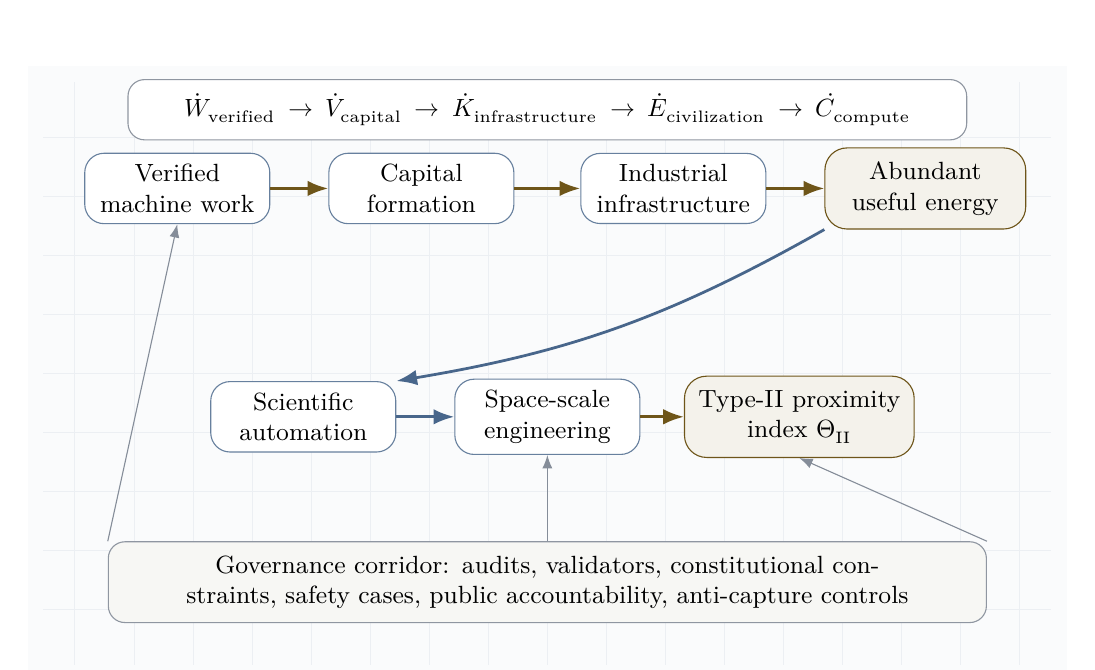
\begin{tikzpicture}[font=\small, >=Latex,
  stage/.style={rounded corners=7pt, draw=AgiBlue!65, fill=white, minimum width=2.35cm, minimum height=0.85cm, align=center, inner sep=4pt},
  horizon/.style={rounded corners=8pt, draw=AgiGold!80!black, fill=AgiGold!9, minimum width=2.55cm, minimum height=0.95cm, align=center, inner sep=5pt},
  guard/.style={rounded corners=6pt, draw=AgiSlate!55, fill=AgiMist, align=center, inner sep=5pt},
  arr/.style={->, line width=1.0pt, AgiBlue!78},
  goldarr/.style={->, line width=1.0pt, AgiGold!80!black}]
\fill[AgiBlue!2] (-6.6,-3.9) rectangle (6.6,3.9);
\draw[AgiBlue!8, line width=0.3pt] (-6.4,-3.7) grid[step=0.75] (6.4,3.7);
\node[stage] (work) at (-4.7,2.35) {Verified\\machine work};
\node[stage] (capital) at (-1.6,2.35) {Capital\\formation};
\node[stage] (industry) at (1.6,2.35) {Industrial\\infrastructure};
\node[horizon] (energy) at (4.8,2.35) {Abundant\\useful energy};
\node[stage] (science) at (-3.1,-0.55) {Scientific\\automation};
\node[stage] (space) at (0,-0.55) {Space-scale\\engineering};
\node[horizon] (typeii) at (3.2,-0.55) {Type-II proximity\\index $\Theta_{\mathrm{II}}$};
\node[guard, text width=10.8cm] (gov) at (0,-2.65) {Governance corridor: audits, validators, constitutional constraints, safety cases, public accountability, anti-capture controls};
\draw[goldarr] (work) -- (capital);
\draw[goldarr] (capital) -- (industry);
\draw[goldarr] (industry) -- (energy);
\draw[arr] (energy.south west) to[bend left=10] (science.north east);
\draw[arr] (science) -- (space);
\draw[goldarr] (space) -- (typeii);
\draw[->,AgiSlate!60] (gov.north west) -- (work.south);
\draw[->,AgiSlate!60] (gov.north) -- (space.south);
\draw[->,AgiSlate!60] (gov.north east) -- (typeii.south);
\node[guard, fill=white, text width=10.3cm] at (0,3.35) {$\dot W_{\mathrm{verified}} \rightarrow \dot V_{\mathrm{capital}} \rightarrow \dot K_{\mathrm{infrastructure}} \rightarrow \dot E_{\mathrm{civilization}} \rightarrow \dot C_{\mathrm{compute}}$};
\end{tikzpicture}

\caption{Civilization-scale value horizon. The system converts verified intelligence work into compounding scientific, industrial, energy, and space capability under a governance corridor.}
\end{figure}

The civilizational objective is:

\[
J_{\mathrm{civil}}(\pi)=
\int_0^T
\left(\Delta W_v+\lambda_E\Delta P_c+\lambda_M\Delta K_m+\lambda_S\Delta K_s\right)dt
-
\int_0^T
\left(\rho R_{\mathrm{cat}}+\mu R_{\mathrm{conc}}+\nu R_{\mathrm{eco}}\right)dt .
\]

\[
\pi^{\star}=\arg\max_{\pi}J_{\mathrm{civil}}(\pi).
\]

subject to:

\[
\text{lawful}\land\text{auditable}\land\text{validator-gated}\land
\text{reversible where possible}\land\text{institutionally governable}.
\]

This is the difference between a powerful swarm and a civilization-grade
engine. A powerful swarm can optimize local objectives. A
civilization-grade engine must transform verified work into durable
public infrastructure: better science, safer energy systems, more
reliable manufacturing, stronger institutions, and space-scale
construction capacity. The value target is therefore not narrow
extraction. It is compounding, governed capability.

The key implication for AGI ALPHA is that the agentic work engine must be
designed as an \textbf{infrastructure multiplier}. Its highest-value
outputs are not only answers, code, or plans, but validated capability
loops that expand humanity's ability to safely command energy, matter,
computation, and coordination. In this sense, $\alpha$-AGI Ascension
becomes a disciplined path from multi-agent work to star-scale
civilizational potential.

\section{Operational architecture}\label{operational-architecture}

A production-grade $\alpha$-AGI work engine requires nine layers.

\subsection{1. Gradient detection layer}\label{gradient-detection-layer}

Detects opportunities, anomalies, research gaps, user needs, software
defects, security events, or market inefficiencies.

\[
g_t=\nabla_{\text{world}}V.
\]

\subsection{2. Job specification layer}\label{job-specification-layer}

Converts gradients into measurable jobs with success criteria,
constraints, risk class, budget, and stopping conditions.

\subsection{3. Agent registry layer}\label{agent-registry-layer}

Maintains agent capabilities, tool permissions, provenance, identity,
reputation, and prior performance.

\subsection{4. Constellation routing
layer}\label{constellation-routing-layer}

Selects agent coalitions by minimizing \(\mathcal{H}(A,j)\) under budget
and risk constraints.

\subsection{5. Execution layer}\label{execution-layer}

Runs tool use, planning, coding, research, simulation, retrieval,
negotiation, and deployment in bounded environments.

\subsection{6. Validation layer}\label{validation-layer}

Applies unit tests, formal checks, human review, adversarial review,
outcome checks, safety filters, and acceptance criteria.

\subsection{7. Settlement layer}\label{settlement-layer}

Allocates reward, reputation, penalties, and future routing probability
according to counterfactual contribution.

\subsection{8. Memory layer}\label{memory-layer}

Stores reusable artifacts, proof traces, errors, policies, tool
outcomes, calibration data, and incident histories.

\subsection{9. Governance layer}\label{governance-layer}

Defines permissions, escalation rules, audit requirements, legal
constraints, red-team procedures, and shutdown modes.

\begin{figure}
\centering
\resizebox{0.88\textwidth}{!}{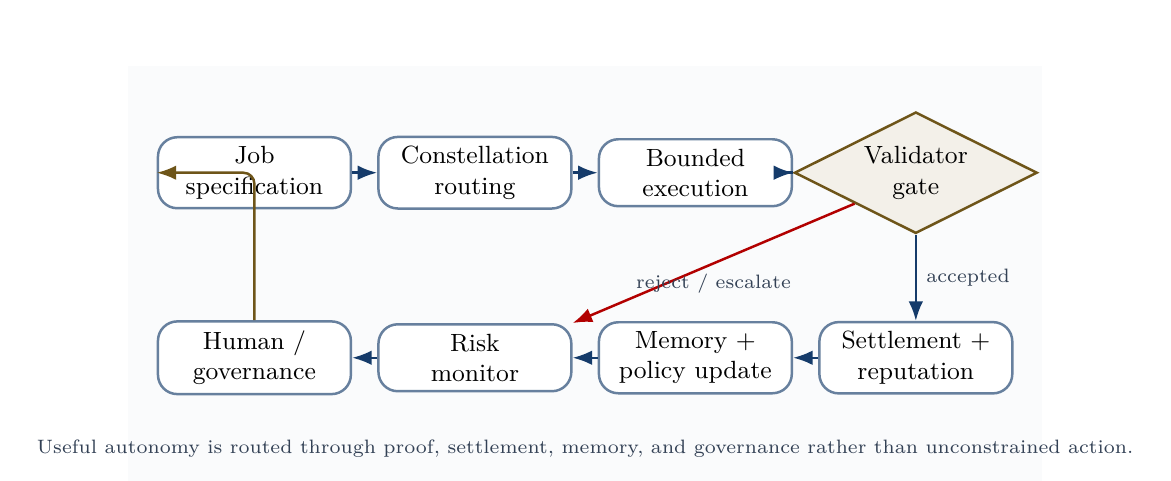
\begin{tikzpicture}[font=\small, >=Latex, line width=0.9pt,
  box/.style={rounded corners=7pt, draw=AgiBlue!65, fill=white, minimum width=2.45cm, minimum height=0.85cm, align=center},
  gate/.style={diamond, aspect=2.0, draw=AgiGold!80!black, fill=AgiGold!10, align=center, inner sep=2pt},
  lab/.style={font=\scriptsize, text=AgiSlate}]
\fill[AgiBlue!2] (-5.8,-2.7) rectangle (5.8,2.7);
\node[box] (job) at (-4.2,1.35) {Job\\specification};
\node[box] (route) at (-1.4,1.35) {Constellation\\routing};
\node[box] (exec) at (1.4,1.35) {Bounded\\execution};
\node[gate] (val) at (4.2,1.35) {Validator\\gate};
\node[box] (settle) at (4.2,-1.00) {Settlement +\\reputation};
\node[box] (mem) at (1.4,-1.00) {Memory +\\policy update};
\node[box] (risk) at (-1.4,-1.00) {Risk\\monitor};
\node[box] (human) at (-4.2,-1.00) {Human /\\governance};
\draw[->,AgiBlue] (job) -- (route);
\draw[->,AgiBlue] (route) -- (exec);
\draw[->,AgiBlue] (exec) -- (val);
\draw[->,AgiBlue] (val) -- node[lab,right]{accepted} (settle);
\draw[->,AgiBlue] (settle) -- (mem);
\draw[->,AgiBlue] (mem) -- (risk);
\draw[->,AgiBlue] (risk) -- (human);
\draw[->,AgiGold!80!black,rounded corners] (human.north) |- (job.west);
\draw[->,red!70!black,rounded corners] (val.south west) -- node[lab,below]{reject / escalate} (risk.north east);
\node[font=\scriptsize, align=center, text=AgiSlate] at (0,-2.15) {Useful autonomy is routed through proof, settlement, memory, and governance rather than unconstrained action.};
\end{tikzpicture}
}
\caption{Validator-gated control loop. Useful autonomy is routed through
proof, settlement, memory, risk monitoring, and governance, rather than
unrestricted action.}
\end{figure}

The validator-loop figure gives the operational discipline behind the system: jobs route
into constellations, constellations execute under tool boundaries,
validators decide acceptance, and the outcome updates settlement,
reputation, memory, risk controls, and governance.

\section{Design principles}\label{design-principles}

The following principles translate current agentic guidance into the
physics/game-theoretic model.

\subsection{Principle 1: start with the simplest sufficient agent
topology}\label{principle-1-start-with-the-simplest-sufficient-agent-topology}

OpenAI's practical guidance recommends maximizing a single agent's
capability before adding multi-agent complexity and distinguishes
manager-style patterns from decentralized handoffs {[}11{]}. Anthropic
similarly distinguishes predictable workflows from more autonomous
agents {[}10{]}. In our framework, unnecessary agents increase
\(C_{\text{coord}}\) and \(S_{\text{swarm}}\) without increasing
\(V_{\text{verified}}\).

\subsection{Principle 2: specialize only where specialization lowers
free
energy}\label{principle-2-specialize-only-where-specialization-lowers-free-energy}

Create a specialist agent only if it reduces:

\[
\Delta\mathcal{G}_{\alpha}<0.
\]

That is, the specialist must improve verified value or reduce cost/risk
more than it increases coordination overhead.

\subsection{Principle 3: make tools legible and
bounded}\label{principle-3-make-tools-legible-and-bounded}

Agentic tools should have clear schemas, scoped permissions, validation,
and observability. Ambiguous tools raise security risk and validator
burden. MCP-style tool connectivity can increase capability, but it must
be paired with least privilege, logging, and prompt-injection defenses
{[}12{]}.

\subsection{Principle 4: validate before
settlement}\label{principle-4-validate-before-settlement}

No agent should receive full reward for unvalidated output. Settlement
follows proof:

\[
\text{work}\rightarrow\text{validation}\rightarrow\text{settlement}\rightarrow\text{memory update}.
\]

\subsection{Principle 5: measure risk as an objective
term}\label{principle-5-measure-risk-as-an-objective-term}

Safety, privacy, legal, and security risks must be in the objective, not
external comments after deployment.

\[
\max \mathbb{E}[V_{\text{verified}}]-\lambda C-\rho R-\kappa U.
\]

\subsection{Principle 6: trace the
system}\label{principle-6-trace-the-system}

Tracing is necessary because multi-agent behavior is otherwise difficult
to debug. The trace should capture agent handoffs, tool calls, guardrail
triggers, validation results, and state updates.

\subsection{Principle 7: design for graceful
degradation}\label{principle-7-design-for-graceful-degradation}

The system should degrade from autonomous execution to human review,
then to read-only advice, then to shutdown. Far-from-equilibrium systems
should not fail by accelerating into unsafe action.

\begin{figure}
\centering
\resizebox{0.88\textwidth}{!}{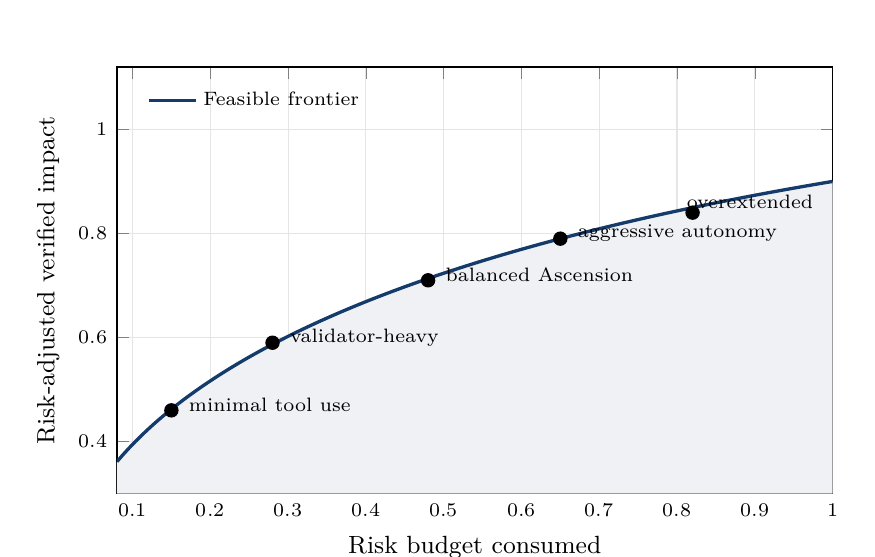
\begin{tikzpicture}
\begin{axis}[
  width=0.88\linewidth,height=7.0cm,
  xmin=0.08,xmax=1.0,ymin=0.3,ymax=1.12,
  xlabel={Risk budget consumed}, ylabel={Risk-adjusted verified impact},
  tick label style={font=\scriptsize}, label style={font=\small},
  legend style={draw=none, fill=none, font=\scriptsize, at={(0.03,0.97)}, anchor=north west},
  grid=both, minor grid style={black!5}, major grid style={black!10}]
\addplot[very thick,AgiBlue, domain=0.08:1.0, samples=120, name path=front] {1.2*sqrt(x)-0.35*x+0.05}; \addlegendentry{Feasible frontier}
\addplot[draw=none, name path=under, domain=0.08:1.0, samples=2] {0.3};
\addplot[fill=AgiBlue!7, draw=none] fill between[of=front and under, soft clip={domain=0.08:1.0}];
\addplot[only marks, mark=*, mark size=2.4pt, black] coordinates {(0.15,0.46) (0.28,0.59) (0.48,0.71) (0.65,0.79) (0.82,0.84)};
\node[font=\scriptsize, anchor=west] at (axis cs:0.16,0.47) {minimal tool use};
\node[font=\scriptsize, anchor=west] at (axis cs:0.29,0.60) {validator-heavy};
\node[font=\scriptsize, anchor=west] at (axis cs:0.49,0.72) {balanced Ascension};
\node[font=\scriptsize, anchor=west] at (axis cs:0.66,0.80) {aggressive autonomy};
\node[font=\scriptsize, anchor=west] at (axis cs:0.80,0.86) {overextended};
\end{axis}
\end{tikzpicture}
}
\caption{Risk-adjusted frontier. The target is not maximum raw autonomy,
but high verified impact under explicit risk budgets.}
\end{figure}

The risk-frontier figure summarizes the governance doctrine: disciplined maximum impact
lives on the frontier where verified value remains high and risk budgets
stay controlled.

\section{Metrics}\label{metrics-5}

\subsection{Verified work efficiency}\label{verified-work-efficiency}

\[
\eta_{\alpha}=\frac{W_{\text{verified}}}{E_{\text{compute}}+C_{\text{human}}+C_{\text{capital}}}.
\]

\subsection{Free-energy descent rate}\label{free-energy-descent-rate}

\[
D_{\mathcal{G}}=-\frac{d\mathcal{G}_{\alpha}}{dt}.
\]

\subsection{Coordination entropy}\label{coordination-entropy}

\[
S_{\text{swarm}}=-\sum_xp(x)\log p(x).
\]

\subsection{Coalition stability}\label{coalition-stability}

\[
K_{\text{coalition}}=\mathbb{E}[\text{lifetime}(A_j)]\cdot\mathbb{E}[\text{success}(A_j)].
\]

\subsection{Credit fidelity}\label{credit-fidelity}

\[
F_{\text{credit}}=\text{corr}(D_i,\Delta r_i).
\]

\subsection{Validator quality}\label{validator-quality}

\[
P_v=\frac{\text{true accepted outputs}}{\text{all accepted outputs}},
\qquad
R_v=\frac{\text{accepted true good outputs}}{\text{all true good outputs}}.
\]

\subsection{Risk-adjusted impact}\label{risk-adjusted-impact}

\[
I_{\text{risk-adjusted}}=V_{\text{verified}}-\rho_sR_{\text{safety}}-\rho_lR_{\text{legal}}-\rho_cR_{\text{security}}.
\]

\subsection{Security loss}\label{security-loss}

\[
L_{\text{security}}=
L_{\text{prompt-injection}}+
L_{\text{tool-abuse}}+
L_{\text{data-leakage}}+
L_{\text{identity-misuse}}+
L_{\text{goal-hijack}}.
\]

\section{Experimental program}\label{experimental-program}

\subsection{Experiment 1: free-energy descent versus verified
work}\label{experiment-1-free-energy-descent-versus-verified-work}

\textbf{Hypothesis.} Constellations selected by minimizing
\(\mathcal{G}_{\alpha}\) produce more verified work per compute unit
than unstructured multi-agent baselines.

\textbf{Conditions.} Compare single-agent, unstructured multi-agent,
role-based multi-agent, and Hamiltonian-routed validator-gated
constellations.

\textbf{Metric.}

\[
\eta_{\alpha}=W_{\text{verified}}/C_{\text{compute}}.
\]

\subsection{Experiment 2: temperature and
exploration}\label{experiment-2-temperature-and-exploration}

\textbf{Hypothesis.} Intermediate effective temperature maximizes
risk-adjusted impact.

\[
T_{\text{low}}\Rightarrow\text{premature convergence}
\]

\[
T_{\text{high}}\Rightarrow\text{coordination noise}
\]

\[
T_{\text{mid}}\Rightarrow\text{productive exploration}.
\]

\subsection{Experiment 3: credit-assignment
fidelity}\label{experiment-3-credit-assignment-fidelity}

\textbf{Hypothesis.} Counterfactual contribution scoring improves agent
selection and reduces reward capture.

Compare:

\[
\Delta r_i=\text{team reward}
\]

against:

\[
\Delta r_i=G(z)-G(z_{-i}).
\]

\subsection{Experiment 4: Hamiltonian coalition
routing}\label{experiment-4-hamiltonian-coalition-routing}

\textbf{Hypothesis.} Learned interaction terms \(J_{ik}\) and
\(K_{ik\ell}\) improve coalition quality over skill-only matching.

\subsection{Experiment 5: validator-gated
safety}\label{experiment-5-validator-gated-safety}

\textbf{Hypothesis.} Validator gating reduces externalized risk without
collapsing useful throughput when validation latency is optimized.

\subsection{Experiment 6: inflow
ablation}\label{experiment-6-inflow-ablation}

\textbf{Hypothesis.} Removing or degrading one continuous inflow creates
a predictable collapse mode.

\begin{itemize}
\tightlist
\item
  Compute ablation: slower loops, under-exploration.
\item
  Data ablation: stale or hallucinated outputs.
\item
  Task ablation: self-referential activity.
\item
  Incentive ablation: low-quality drift.
\item
  Feedback ablation: uncorrected error accumulation.
\item
  Governance ablation: unsafe optimization.
\item
  Tool ablation: low external work.
\end{itemize}

\section{Formal proposition: \texorpdfstring{$\alpha$}{alpha}-AGI Ascension as bounded dissipative
intelligence}\label{formal-proposition-alpha-agi-ascension-as-bounded-dissipative-intelligence}

A large-scale multi-agent system enters an $\alpha$-AGI Ascension regime when:

\begin{enumerate}
\def\labelenumi{\arabic{enumi}.}
\tightlist
\item
  it is open to continuous inflows of compute, data, tasks, incentives,
  feedback, governance, and tools;
\item
  it maintains non-equilibrium organization through specialization and
  coalition formation;
\item
  it converts inflows into externally validated work;
\item
  it dissipates failed search, latency, and redundant computation;
\item
  it updates memory, reputation, and routing from validation outcomes;
\item
  it bounds risk through governance, permissions, and validators.
\end{enumerate}

Formally:

\[
\alpha\text{-Ascension}
\iff
\begin{cases}
\dot{E}_{\text{in}}>0 \\
\dot{W}_{\text{verified}}>0 \\
S_{\min}<S_{\text{swarm}}<S_{\max} \\
R_{\text{safety}}\leq R_{\max} \\
\frac{d\mathcal{G}_{\alpha}}{dt}<0 \\
F_{\text{credit}}\rightarrow 1.
\end{cases}
\]

This is the precise sense in which AGI ALPHA can be said to bring $\alpha$-AGI
Ascension to life.

\section{Discussion}\label{discussion}

The framework should be read as disciplined analogy plus testable
engineering. The physical compute layer is literally thermodynamic:
electrical energy is consumed, processors dissipate heat, and
networks/storage impose physical constraints. The coordination layer is
formal: \(\mathcal{G}_{\alpha}\) is not chemical Gibbs energy, but a
useful state functional over cost, risk, value, and exploration.

The statistical-physics view is useful because large agent swarms are
ensemble systems. It is often impossible to inspect every message or
decision, but possible to measure macro-observables: entropy, risk,
verified output, coalition stability, validator latency, and credit
fidelity.

The Hamiltonian view is useful because interacting learners can cycle.
Purely strategic dynamics may orbit around equilibria without producing
useful work. The missing ingredient is dissipation into validated
artifacts. $\alpha$-AGI should not merely think, debate, or strategize; it
should settle into proof-producing trajectories.

The game-theoretic view is useful because local incentives determine
global structure. If reward follows verbosity, agents become verbose. If
reward follows proof, agents become proof-seeking. If reward follows
unsafe speed, agents become unsafe. Mechanism design is therefore not an
economic add-on; it is part of the physics of the swarm.

\section{Limitations}\label{limitations}

This paper has several limitations.

\begin{enumerate}
\def\labelenumi{\arabic{enumi}.}
\tightlist
\item
  \(\mathcal{G}_{\alpha}\) is an engineered objective, not a natural
  thermodynamic state variable.
\item
  Hamiltonian parameters must be learned, estimated, or manually
  specified.
\item
  Validators may become bottlenecks, attack targets, or sources of bias.
\item
  Counterfactual credit assignment is approximate and can be gamed.
\item
  Multi-agent communication creates privacy, security, collusion, and
  hallucination risks.
\item
  ``Maximum impact'' is a normative target and cannot be defined by
  throughput, profit, or autonomy alone.
\item
  Empirical claims require benchmark results, deployment traces, and
  independent audits.
\end{enumerate}

\section{Conclusion}\label{conclusion}

AGI ALPHA can be scientifically framed as a far-from-equilibrium
multi-agent work engine. $\alpha$-AGI Ascension is the sustained regime in
which compute, data, tasks, incentives, feedback, governance, and tools
maintain organized agentic complexity and convert it into externally
verified impact.

The final formulation is:

\[
\boxed{
\begin{aligned}
\alpha\text{-AGI Ascension}
=&\;\arg\min_{\text{agent constellations}}\;[\,C_{\text{compute}}+C_{\text{coordination}}\\
&+R_{\text{safety}}-V_{\text{verified}}-T_{\text{eff}}S_{\text{useful exploration}}\,]
\end{aligned}}
\]

sustained by:

\[
\boxed{
\dot{E}_{\text{compute,data,capital,tasks}}
\rightarrow
\dot{W}_{\text{verified impact}}
+
\dot{Q}_{\text{dissipated search}}
+
\dot{I}_{\text{memory}}
}
\]

and constrained by:

\[
\boxed{
\text{lawful}\land\text{auditable}\land\text{permissioned}\land\text{validator-gated}\land\text{risk-bounded}.
}
\]

Thus, the strongest scientific version of the claim is:

\textbf{AGI ALPHA brings $\alpha$-AGI Ascension to life by engineering
dissipative intelligence: a continuously powered, statistically mapped,
Hamiltonian-routed, game-theoretically aligned, validator-gated swarm
that transforms energy-mediated computation into verified impact.}

\section{Appendix A: variable
glossary}\label{appendix-a-variable-glossary}

\begin{longtable}[]{@{}ll@{}}
\toprule\noalign{}
Symbol & Meaning \\
\midrule\noalign{}
\endhead
\bottomrule\noalign{}
\endlastfoot
\(\mathcal{A}\) & Agent population \\
\(\mathcal{J}\) & Job stream \\
\(\Phi_C\) & Compute inflow \\
\(\Phi_D\) & Data inflow \\
\(\Phi_J\) & Task/job inflow \\
\(\Phi_I\) & Incentive inflow \\
\(\Phi_F\) & Feedback inflow \\
\(\Phi_G\) & Governance inflow \\
\(\Phi_T\) & Tool/environment inflow \\
\(\mathcal{G}_{\alpha}\) & Agentic Gibbs-like free-energy functional \\
\(\mathcal{H}\) & Hamiltonian-like cost of a configuration \\
\(S_{\text{swarm}}\) & Entropy of swarm configurations \\
\(V_{\text{verified}}\) & Externally validated value \\
\(R_{\text{safety}}\) & Safety risk \\
\(D_i\) & Counterfactual contribution of agent \(i\) \\
\(P_v\) & Validator precision \\
\(R_v\) & Validator recall \\
\(\Theta_{\mathrm{II}}\) & Type-II / star-scale proximity index \\
\(P_{\text{controlled}}\) & Sustainably governed useful power \\
\(L_{\star}\) & Host-star luminosity benchmark \\
\end{longtable}

\section{Appendix B: operational inflow
checklist}\label{appendix-b-operational-inflow-checklist}

\begin{longtable}[]{@{}
  >{\raggedright\arraybackslash}p{(\columnwidth - 4\tabcolsep) * \real{0.3333}}
  >{\raggedright\arraybackslash}p{(\columnwidth - 4\tabcolsep) * \real{0.3333}}
  >{\raggedright\arraybackslash}p{(\columnwidth - 4\tabcolsep) * \real{0.3333}}@{}}
\toprule\noalign{}
\begin{minipage}[b]{\linewidth}\raggedright
Layer
\end{minipage} & \begin{minipage}[b]{\linewidth}\raggedright
Minimum viable control
\end{minipage} & \begin{minipage}[b]{\linewidth}\raggedright
Production-grade control
\end{minipage} \\
\midrule\noalign{}
\endhead
\bottomrule\noalign{}
\endlastfoot
Compute & Token/tool budget & Dynamic budgets, sandboxing, energy
accounting \\
Data & Source links & Provenance graph, freshness scoring, poisoning
defense \\
Tasks & Written objective & Formal success criteria, risk class,
stopping rule \\
Incentives & Bounty & Counterfactual contribution settlement \\
Feedback & Manual approval & Multi-validator feedback with
calibration \\
Governance & Basic policy & Lifecycle risk management and audit
trails \\
Tools & API access & Least-privilege scoped tools with approval gates \\
Memory & Conversation history & Versioned, permissioned,
provenance-tagged memory \\
Security & Basic filtering & Threat model, red team, incident response,
identity controls \\
\end{longtable}


\section{Appendix C: AGI Alpha doctrine corpus map}\label{appendix-c-doctrine-corpus}

The supplied Vincent Boucher corpus was considered as an institutional
strategy corpus. The paper does not reproduce or rely on long quotations;
it distills recurring architectural commitments into a scientific control
framework.

\begin{longtable}[]{@{}>{\raggedright\arraybackslash}p{0.26\linewidth}>{\raggedright\arraybackslash}p{0.34\linewidth}>{\raggedright\arraybackslash}p{0.32\linewidth}@{}}
\toprule
Doctrine theme & Representative corpus signals & Paper-level translation \\
\midrule
\endhead
AI sovereignty & AGI-driven labor engine, decentralized AGI labor platform, sovereign machine, republic of machines & Institutional capacity to command verifiable synthetic labor under local governance. \\
Agent-native economy & Agent-native sales, machine-to-machine economy, global marketplace of sovereign agents & Markets where agents discover, bid, execute, prove, settle, and update reputation. \\
On-chain work and settlement & AGIJobManager, AGIJobManagerPrime, DiscoveryPrime, ENS job pages, no judge but code & Proof-bearing jobs, validator-gated escrow, identity, settlement, and public memory. \\
Autonomous capital & Autonomous agents closing loops, capital becoming autonomous, self-sustaining digital firms & Reinvestment loops that convert verified work into capital, infrastructure, and compute. \\
Tournament and proof & Proof of Talent, Tournament for Intelligence, Selection Chamber & Competitive routing and counterfactual credit assignment for intelligent labor. \\
Recursive improvement governance & AGI Alpha RSI, sovereign invention governance, verified autonomy control plane & Improvement under audit, permissions, logging, rollback, and constitutional constraints. \\
Civilizational horizon & Machine labor at planetary scale, invention market, machine buying the sun & Verified work compounding into scientific capability, abundant energy, and infrastructure. \\
\bottomrule
\end{longtable}

\section{References}\label{references}

{[}1{]} Nobel Prize. ``The Nobel Prize in Chemistry 1977 - Press
release: Ilya Prigogine.'' NobelPrize.org, 1977.
\url{https://www.nobelprize.org/prizes/chemistry/1977/press-release/}

{[}2{]} OpenStax. ``16.4 Free Energy.'' \emph{Chemistry 2e}, 2019.
\url{https://openstax.org/books/chemistry-2e/pages/16-4-free-energy}

{[}3{]} Jaynes, E. T. ``Information Theory and Statistical Mechanics.''
\emph{Physical Review} 106, 620-630, 1957.
\url{https://link.aps.org/doi/10.1103/PhysRev.106.620}

{[}4{]} Bailey, James P., and Georgios Piliouras. ``Multi-Agent Learning
in Network Zero-Sum Games is a Hamiltonian System.'' arXiv:1903.01720,
2019. \url{https://arxiv.org/abs/1903.01720}

{[}5{]} Guo, Taicheng, et al.~``Large Language Model based Multi-Agents:
A Survey of Progress and Challenges.'' arXiv:2402.01680, 2024.
\url{https://arxiv.org/abs/2402.01680}

{[}6{]} Yan, Bingyu, et al.~``Beyond Self-Talk: A Communication-Centric
Survey of LLM-Based Multi-Agent Systems.'' arXiv:2502.14321, 2025.
\url{https://arxiv.org/abs/2502.14321}

{[}7{]} Li, Xinyi, et al.~``A survey on LLM-based multi-agent systems:
workflow, infrastructure, and challenges.'' \emph{Vicinagearth} 1, 9,
2024. \url{https://link.springer.com/article/10.1007/s44336-024-00009-2}

{[}8{]} NIST. ``Artificial Intelligence Risk Management Framework:
Generative Artificial Intelligence Profile (NIST AI 600-1).'' 2024.
\url{https://www.nist.gov/publications/artificial-intelligence-risk-management-framework-generative-artificial-intelligence}

{[}9{]} OWASP GenAI Security Project. ``Agentic AI - Threats and
Mitigations'' and ``Securing Agentic Applications Guide 1.0.'' 2025.
\url{https://genai.owasp.org/resource/agentic-ai-threats-and-mitigations/} ;
\url{https://genai.owasp.org/resource/securing-agentic-applications-guide-1-0/}

{[}10{]} Anthropic. ``Building Effective AI Agents.'' 2024.
\url{https://www.anthropic.com/research/building-effective-agents}

{[}11{]} OpenAI. ``A practical guide to building agents'' and ``Agents
SDK.'' 2025-2026.
\url{https://openai.com/business/guides-and-resources/a-practical-guide-to-building-ai-agents/}
; \url{https://developers.openai.com/api/docs/guides/agents}

{[}12{]} Model Context Protocol. ``Specification.'' 2025.
\url{https://modelcontextprotocol.io/specification/2025-11-25}

{[}13{]} Sunehag, Peter, et al.~``Value-Decomposition Networks For
Cooperative Multi-Agent Learning.'' arXiv:1706.05296, 2017.
\url{https://arxiv.org/abs/1706.05296}

{[}14{]} Friston, Karl, et al.~``The free energy principle made simpler
but not too simple.'' arXiv:2201.06387, 2022.
\url{https://arxiv.org/abs/2201.06387}

{[}15{]} Ruiz-Serra, Jaime, Patrick Sweeney, and Michael S. Harre.
``Factorised Active Inference for Strategic Multi-Agent Interactions.''
arXiv:2411.07362, 2024. \url{https://arxiv.org/abs/2411.07362}

{[}16{]} MontrealAI. ``AGI-Alpha-Agent-v0: $\alpha$-AGI Architect -
Foundational Operational Blueprint.'' GitHub repository.
\url{https://github.com/MontrealAI/AGI-Alpha-Agent-v0}


[17] Kardashev, N. S. ``Transmission of Information by Extraterrestrial
Civilizations.'' \emph{Soviet Astronomy} 8, 217-221, 1964.

[18] Dyson, Freeman J. ``Search for Artificial Stellar Sources of
Infrared Radiation.'' \emph{Science} 131, no. 3414, 1667-1668, 1960.
\url{https://doi.org/10.1126/science.131.3414.1667}


[19] MontrealAI. "AGI-Alpha-Agent-v0: META-AGENTIC alpha-AGI." GitHub repository. \url{https://github.com/MontrealAI/AGI-Alpha-Agent-v0}

[20] MontrealAI. "MONTREAL.AI / Montreal Artificial Intelligence." GitHub profile. \url{https://github.com/MontrealAI}

[21] MONTRÉAL.AI. "We Choose to Ascend with AGI." Public institutional page and AGI Jobs overview. \url{https://montrealai.github.io/}

[22] Vincent Boucher. "Featured writings on AI sovereignty, agent-native economy, AGI Alpha, sovereign agents, on-chain governance, public memory, proof of talent, autonomous capital, recursive improvement, and civilizational-scale machine labor." LinkedIn featured corpus. \url{https://www.linkedin.com/in/montrealai/details/featured/}

[23] Etherscan. "AGIJobManager, ENSJobPages, AGIJobDiscoveryPrime, AGIJobManagerPrime, and AGI ALPHA AGENT (AGIALPHA) public contract pages." Ethereum contract explorer. \url{https://etherscan.io/}



[24] Xu, Jinglue, et al. "TRINITY: An Evolved LLM Coordinator." arXiv:2512.04695, 2025. \url{https://arxiv.org/abs/2512.04695}

[25] Dang, Yufan, et al. "Multi-Agent Collaboration via Evolving Orchestration." NeurIPS 2025 / OpenReview, 2025. \url{https://openreview.net/pdf/9727f658d788c52f49f12ae4b230baf4cf0d4007.pdf}

[26] Chi, Zewen, et al. "The Era of Agentic Organization: Learning to Organize with Language Models." arXiv:2510.26658, 2025. \url{https://arxiv.org/abs/2510.26658}

[27] Hua, Keru, et al. "DUPLEX: Agentic Dual-System Planning via LLM-Driven Information Extraction." arXiv:2603.23909, 2026. \url{https://arxiv.org/abs/2603.23909}

[28] Zong, Zefang, et al. "AT$^2$PO: Agentic Turn-based Policy Optimization via Tree Search." arXiv:2601.04767, 2026. \url{https://arxiv.org/abs/2601.04767}

[29] Sun, Mingyang, Feng Hong, and Weinan Zhang. "Sophia: A Persistent Agent Framework of Artificial Life." arXiv:2512.18202, 2025. \url{https://arxiv.org/abs/2512.18202}

[30] Wei, Yuxiang, et al. "Toward Training Superintelligent Software Agents through Self-Play SWE-RL." arXiv:2512.18552, 2025. \url{https://arxiv.org/abs/2512.18552}

[31] Wang, Wenyi, et al. "Huxley-Gödel Machine: Human-Level Coding Agent Development by an Approximation of the Optimal Self-Improving Machine." arXiv:2510.21614, 2025. \url{https://arxiv.org/abs/2510.21614}

[32] Wang, Yiping, et al. "ThetaEvolve: Test-time Learning on Open Problems." arXiv:2511.23473, 2025. \url{https://arxiv.org/abs/2511.23473}

[33] Wolchover, Natalie. "What Physical 'Life Force' Turns Biology's Wheels?" Quanta Magazine, 2026. \url{https://www.quantamagazine.org/what-physical-life-force-turns-biologys-wheels-20260420/}

[34] Darlow, Luke. "Digital Ecosystems: Interactive Multi-Agent Neural Cellular Automata." Sakana AI, 2026. \url{https://pub.sakana.ai/digital-ecosystem/}

[35] Tomašev, Nenad, et al. "Distributional AGI Safety." arXiv:2512.16856, 2025. \url{https://arxiv.org/abs/2512.16856}

[36] Tomašev, Nenad, et al. "Virtual Agent Economies." arXiv:2509.10147, 2025. \url{https://arxiv.org/abs/2509.10147}

[37] Mahadevan, Sridhar. "Large Causal Models from Large Language Models." arXiv:2512.07796, 2025. \url{https://arxiv.org/abs/2512.07796}

[38] Li, Orion, et al. "K-Dense Analyst: Towards Fully Automated Scientific Analysis." arXiv:2508.07043, 2025. \url{https://arxiv.org/abs/2508.07043}

[39] Guo, Yiduo, et al. "Synthetic Data RL: Task Definition Is All You Need." arXiv:2505.17063, 2025. \url{https://arxiv.org/abs/2505.17063}

[40] Rector-Brooks, Jarrid, et al. "General Multimodal Protein Design Enables DNA-Encoding of Chemistry." arXiv:2604.05181, 2026. \url{https://arxiv.org/abs/2604.05181}

[41] Liu, Yixiu, et al. "AlphaGo Moment for Model Architecture Discovery." arXiv:2507.18074, 2025. \url{https://arxiv.org/abs/2507.18074}

[42] Chen, Qiguang, et al. "The Molecular Structure of Thought: Mapping the Topology of Long Chain-of-Thought Reasoning." arXiv:2601.06002, 2026. \url{https://arxiv.org/abs/2601.06002}

[43] Shafayat, Sheikh, et al. "Can Large Reasoning Models Self-Train?" arXiv:2505.21444, 2025. \url{https://arxiv.org/abs/2505.21444}

\end{document}
